\documentclass{beamer}
% ---- Minimal setup (XeLaTeX) ----
\usepackage{fontspec}
\defaultfontfeatures{Ligatures=TeX}
%\usepackage{luatexja}
%\usepackage{luatexja-fontspec}
%\ltjsetparameter{jacharrange={-9}}
\setmainfont{TeX Gyre Pagella}
\setsansfont{TeX Gyre Heros}
\setmonofont{Inconsolata} % TeX Gyre Cursor} %  Fira Mono}
% Auto-switch by Unicode block
% Font families for non-Latin scripts
\newfontfamily\jafont{Noto Sans CJK JP}
\newfontfamily\krfont{Noto Sans CJK KR}
\newfontfamily\hanfont{Noto Sans CJK SC}
\newfontfamily\devanagarifont{Noto Sans Devanagari}
\newfontfamily\ipafont{Gentium}

% Explicit font-switching macros — use these to wrap non-Latin text
\newcommand{\ja}[1]{{\jafont #1}}          % Japanese
\newcommand{\cn}[1]{{\hanfont #1}}         % Chinese/Mandarin
\newcommand{\ko}[1]{{\krfont #1}}          % Korean
\newcommand{\dv}[1]{{\devanagarifont #1}}  % Devanagari
\newcommand{\ipa}[1]{{\ipafont #1}}        % IPA
\newcommand{\jpf}[1]{\ja{#1}}             % backward-compat alias

% Graceful fallback in PDF bookmarks
\pdfstringdefDisableCommands{%
  \def\ja#1{#1}%
  \def\cn#1{#1}%
  \def\ko#1{#1}%
  \def\dv#1{#1}%
  \def\ipa#1{#1}%
  \def\jpf#1{#1}%
}
% \newfontfamily\emoji{Noto Color Emoji}[Renderer=Harfbuzz,Scale=MatchLowercase]
% \newcommand{\e}[1]{{\emoji #1}}

\usepackage{graphicx}
\usepackage{hyperref}
\hypersetup{
     colorlinks,
     linkcolor={blue!50!black},
     citecolor={red!50!black},
     urlcolor={blue!80!black}
   }
\usepackage{booktabs}
\usepackage{microtype}

\newcommand{\txx}[1]{\textbf{\textcolor{blue}{#1}}}

% --- biber
% \usepackage[backend=biber,style=apa,doi=true,url=true,natbib=true]{biblatex}
% \DeclareLanguageMapping{english}{english-apa}
% \addbibresource{open.bib}
\usepackage[round]{natbib}

% ---- Beamer look ----
\usetheme{Boadilla}
\usecolortheme{seahorse}
\setbeamertemplate{navigation symbols}{}
\setbeamertemplate{itemize items}[circle]
\setbeamertemplate{itemize subitem}[triangle]
%\setbeamertemplate{footline}[frame number]
\setbeamerfont{block body example}{size=\small}
\setbeamerfont{block title example}{size=\small}  % optional: adjust title too
% ---- Section outline slide ----
\AtBeginSection[]{
  \begin{frame}
    \frametitle{Roadmap}
    \small
    \tableofcontents[currentsection, hideothersubsections]%, hideallsubsections]
  \end{frame}
}
\logo{
\includegraphics[width=15mm]{img/UP_logo_FF_horizont_en.png}}

% ---- other packages
\usepackage{tikz}

% ---- Linguistics

\usepackage{langsci-gb4e}
\usepackage{avm}

\usepackage[normalem]{ulem}
\newcommand{\ul}{\uline}
\newcommand{\ull}{\uuline}
\newcommand{\udl}{\dashuline}
\newcommand{\uwl}{\uwave}

\usepackage[e,f,j]{mtg2e}
\newcommand{\cmn}{\mtciteform}
\newcommand{\kor}{\mtciteform}
\renewcommand{\mtcitestyle}[1]{\textcolor{teal}{\textit{#1}}}
\usepackage{xcolor}
 \newcommand{\bs}{\textbackslash}   % backslash
 \newcommand{\cmd}[1]{{\bf \color{red}#1}}   % highlights command
 \newcommand{\wemp}[1]{\ul{#1}}   % highlight
 \newcommand{\emp}[1]{\textbf{\color{blue}{#1}}}   % highlight
 \newcommand{\rel}[1]{\textsc{\color{blue}{#1}}}
 %%% imi zokusei
 \newcommand{\iz}[1]{\textup{\texttt{\color{blue}{\textbf{#1}}}}}
 \newcommand{\con}{\iz}
 \newcommand{\lnk}[1]{\rel{#1}}
 \newcommand{\dff}[1]{\rel{#1}}
\newcommand{\cmp}[1]{{[\textsc{#1}]}}
\newcommand{\elem}[1]{\ensuremath{\langle}\texttt{#1}\ensuremath{\rangle}}
 \newcommand{\lex}[1]{\textbf{\color{teal}{\textit{#1}}}}
 \newcommand{\lng}[1]{\textcolor{teal}{\textit{#1}}}
\newcommand{\wn}[3]{\lex{#1}\ensuremath{_{#2:#3}}}
\usepackage{relsize,xspace}
\newcommand{\wnida}[1]{\asort{\wnid{#1}}}
\newcommand{\wnid}[1]{\textsf{\smaller #1}}
\newcommand{\topic}[1]{\textsc{#1}}
\newcommand{\into}{\ensuremath{\rightarrow}\xspace}
\newcommand{\ent}{\ensuremath{\Rightarrow}\xspace}
\newcommand{\nent}{\ensuremath{\not\Rightarrow}\xspace}
\newcommand{\tot}{\ensuremath{\leftrightarrow}\xspace}

\newcommand{\MyLogo}[1]{}

% \newcommand{\task}{\marginpar{\raisebox{-2ex}{
%       \hspace{-0.5em}\reflectbox{\includegraphics[width=2em]{img/detective.pdf}}}}}
\newcommand{\task}{?}


\setbeamercolor{taskc}{fg=black,bg=red!10}

\newenvironment{taskb}[1][]{%
  \begin{beamercolorbox}[rounded=true,shadow=true,wd=\linewidth,sep=0.5em]{taskc}
    \ifx\relax#1\relax
      % No title - just show content
    \else
      % Title provided
      \textbf{\large ?} #1
      \par\vspace{0.3em}
    \fi
}{%
  \end{beamercolorbox}
  \vspace{0.5em}
}


\title[Open Multilingual Wordnet]{Methods in Lexical Semantics: 
\\ Multilingual WordNets and Lexical Structure}
%\\[2ex] \bl{Picking Brains, Crossing Ideas}}
\author{Francis \textbf{Bond}}
\institute[Palacký]{Department of Asian Studies,
\\  Palacký University, Olomouc, Czechia
\\[1.5ex] \url{<bond@ieee.org>}}


\date{University of Ljubljana, April 2026}
\newcommand{\ili}[1]{\href{http://www.globalwordnet.org/ili/#1}{\url{#1}}}

% %\usepackage[hidelinks]{hyperref}
% \hypersetup{ 
%      colorlinks,
%      linkcolor={blue!50!black},
%      citecolor={red!50!black},
%      urlcolor={blue!80!black}
% }


\usepackage{array}
\newcolumntype{H}{>{\setbox0=\hbox\bgroup}c<{\egroup}@{}}

\usepackage{forest}
\newcommand{\wnbox}[1]{\parbox[t]{24em}{#1}}

% \usepackage[round]{natbib}
% \usepackage{fontenc}
% \usepackage{polyglossia}
% \setmainlanguage{english}
% \usepackage{xeCJK}
% %\setCJKmainfont{WenQuanYi Micro Hei}
% % \setmainfont[Numbers=OldStyle]{TeX Gyre Pagella}
% %\setCJKmainfont{Droid Sans Fallback}
% \setCJKmainfont{Noto Sans CJK SC}
% \usefonttheme{professionalfonts}
% \setsansfont{Linux Libertine O}
% \logo{NTU}
% \logo{
\includegraphics[width=15mm]{img/UP_logo_FF_horizont_en.png}}


\newcommand{\zhong}{\ensuremath{[\Big|]}}
% NUS Meeting Room 1 (MR 1) 	COM1-03-19
\newcommand{\bl}[1]{\textcolor{blue}{#1}}
%\newcommand{\sh}[1]{\textcolor{blue}{#1}}
%\newcommand{\txx}[1]{\textbf{\textcolor{blue}{#1}}}
\usepackage{url}

%\newcommand{\wn}{\url}

%\newcommand{\MyLogo}[1]{(#1)}

% \newcommand{\sh}[1]{https://fcbond.github.io/sh-canon/#1.html}
% \newcommand{\SCAN}{\href{\sh{scan}}{\textit{A Scandal in Bohemia}}\xspace}
% \newcommand{\REDH}{\href{\sh{redh}}{\textit{The Redheaded League}}\xspace}
% \newcommand{\HOUN}{\href{\sh{houn}}{\textit{The Hound of the
%       Baskervilles}}\xspace}
% \newcommand{\SPEC}{\href{\sh{spec}}{\textit{The Adventure of the Speckled Band}}\xspace}
% \newcommand{\DANC}{\href{\sh{danc}}{\textit{The Adventure of the Dancing Men}}\xspace}
% \newcommand{\FINA}{\href{\sh{fina}}{\textit{The Adventure of the Final Problem}}\xspace}
% \newcommand{\NAVA}{\href{\sh{nava}}{\textit{The Adventure of the Naval Treaty}}\xspace}

\newcommand{\swn}{SentiWordNet\xspace}
\newcommand{\plwn}{plWordNet\xspace}
\newcommand{\plemo}{plWordNet~emo\xspace}
\newcommand{\pwn}{Princeton WordNet\xspace} 
\newcommand{\mlsc}{ML-SentiCon\xspace}
\newcommand{\wnop}{\textsc{Micro-WNOp}\xspace}
\newcommand{\ntumc}{NTU-MC\xspace}

% typesetting: metaphors
\newcommand{\defn}[1]{{\textbf{#1}}}
\newcommand{\metaphor}[1]{\textsc{#1}}
\newcommand{\word}[1]{\textit{#1}}
\newcommand{\concept}[1]{\textsc{#1}}
\newcommand{\letter}[1]{\texttt{#1}}
\newcommand{\sense}[2]{\word{#1}\textsubscript{$#2$}}
\newcommand{\synonym}[1]{\textit{#1}}


\newcommand{\tabspace}{\addlinespace[0.6em]}
\newcommand{\slipspace}{\addlinespace[0.1em]}
\newcommand{\tighteq}{\,{=}\,}

\usepackage{adjustbox}
\usepackage{array}
\usepackage{tikz}

\newcommand{\literalcolour}{Brown}
\newcommand{\relatedcolour}{Bittersweet}
\newcommand{\metaphoricalcolour}{Purple}
\newcommand{\conduitcolour}{Gray}

\newcommand{\literallabel}{Prototype}
\newcommand{\relatedlabel}{Associated}
\newcommand{\metaphoricallabel}{Metaphorical}
\newcommand{\relatededgelabel}{Metonymy}
\newcommand{\relatededgelabelshort}{Meton.}
\newcommand{\metaphoricaledgelabel}{Metaphor}
\newcommand{\conduitlabel}{{ }+{ }Conduit}
\newcommand{\conduitmetlabel}{\hphantom{\metaphoricallabel}\conduitlabel}
\newcommand{\conduitasslabel}{\hphantom{\relatedlabel}\conduitlabel}

\newcolumntype{R}[2]{%
    >{\adjustbox{angle=#1,lap=\width-(#2)}\bgroup}%
    l%
    <{\egroup}%
}
\newcommand*\rot{\multicolumn{1}{R{30}{1.5em}}}

\newcommand{\literal}{\makecell{\textcolor{\literalcolour}{\literallabel}}}
\newcommand{\related}[2]{\makecell{\textcolor{\relatedcolour}{\relatedlabel} \\ \textcolor{\relatedcolour}{(from \sense{#1}{#2})}}}
\newcommand{\onlymetaphorical}{\makecell{\textcolor{\metaphoricalcolour}{\metaphoricallabel}}}
\newcommand{\metaphorical}[2]{\makecell{\textcolor{\metaphoricalcolour}{\metaphoricallabel} \\ \textcolor{\metaphoricalcolour}{(from \sense{#1}{#2})}}}
\newcommand{\feature}[1]{\scalebox{.8}[1.0]{\texttt{#1}}}
\newcommand{\yesfeature}[1]{\textcolor{Green}{\feature{#1}}}
\usepackage[normalem]{ulem}
\newcommand{\nofeature}[1]{\textcolor{Red}{\sout{\feature{#1}}}}
\newcommand{\maybefeature}[2]{\textcolor{Green}{\feature{#1}} \textcolor{Orange}{\feature{#2}}}
\newcommand{\allmaybefeature}[1]{\textcolor{Orange}{\feature{#1}}}
\newcommand{\defaultdepth}{0pt}
\tikzset{definition/.style={align=left, shape=rectangle,draw=black, font={\footnotesize}, fill=black!0!white}}
\tikzset{invis/.style={align=left, shape=rectangle,draw=none, font={\footnotesize}, fill=none,text opacity=0}}
\tikzset{lit_definition/.style={anchor=center, align=left, shape=rectangle,draw=\literalcolour, font={\footnotesize}, label={[label distance=-.05cm]:{\footnotesize{\textcolor{\literalcolour}{\literallabel}}}}, fill=black!0!white}}
\tikzset{met_definition/.style={align=left, shape=rectangle,draw=\metaphoricalcolour, font={\footnotesize}, fill=black!0!white}}
\tikzset{ass_definition/.style={align=left, shape=rectangle,draw=\relatedcolour, font={\footnotesize}, fill=black!0!white}}
\tikzset{ghost/.style={ass_definition, dashed}}
\tikzset{ghost_core/.style={lit_definition, dashed}}

% , on layer=bg
\tikzset{split/.style={-, dashed, line width=.3mm, Gray}}
\tikzset{start/.style={->, line width=.3mm, \literalcolour}}
\tikzset{analogy/.style={->, line width=.3mm, \metaphoricalcolour}}
\tikzset{related/.style={->, line width=.3mm, \relatedcolour}}
\tikzset{unknown/.style={->, line width=.3mm}}

\tikzset{derivation/.style={node distance = .7cm and %1.9cm}}
1cm}}
\tikzset{tight/.style={node distance = .55cm and .5cm}}
\tikzset{close/.style={node distance = .6cm and %1.9cm}}
.3cm}}

\newenvironment{tightcenter}{%
  \setlength\topsep{0pt}
  \setlength\parskip{0pt}
  \begin{center}
}{%
  \end{center}
}

\newcommand{\featuregoesto}{\textcolor{\metaphoricalcolour}{$\rightarrow$}}
% space hacks
\setlength{\belowcaptionskip}{-5pt}
\everypar{\looseness=-1}

\usepackage{tikz}
\usepackage{tikz-dependency}
\newcommand{\horn}[1]{\ensuremath{\langle}\lex{#1}\ensuremath{\rangle}}

\usepackage{tikz-qtree}


\begin{document}
\maketitle
%\lingset{lingstyle=cmn}
\begin{frame}{Outline}
   \tableofcontents
 \end{frame}


% \begin{frame}{Self Introduction}

% \begin{itemize}\addtolength{\itemsep}{-0.5ex}
% %\item Francis Bond 
% \item BA in Japanese and Mathematics 
%   \hfil\raisebox{-4.5ex}[0mm][0mm]{
\includegraphics[width=5em]{pwm.pdf}}
% \item BEng in Power and Control %(Electrical Systems Engineering)

% \item PhD in English on  \textit{Determiners and Number in English
%   contrasted with Japanese,  as exemplified in Machine
%   Translation} 
% \item 1991-2006 NTT (Nippon Telegraph and Telephone)
%   \begin{itemize}
%   \item Japanese - English/Malay Machine Translation
%   \item Japanese corpus, HPSG grammar and ontology (Hinoki)
%   \end{itemize}
% \item 2006-2009 NICT (National Inst. for Info. and Comm. Technology)
%   \begin{itemize}
%   \item Japanese - English/Chinese Machine Translation
%   \item Japanese WordNet
%   \end{itemize}
% \item 2009- NTU (Nanyang Technological University)
%   \begin{itemize}
%   \item Abui, Chinese, Malay, Multilingual Wordnets
%   \item HPSGs for Chinese, Indonesian, \ldots
%   \item Multilingual Meaning Banks (Treebank + Sensebank)
%   \end{itemize}

% \end{itemize}
% \end{frame}
  
\section{Wordnets in the World}
\begin{frame}{WordNet (revision)}

%\MyLogo{\citet{Miller:1998:foreword,_Fellbaum:1998}}

\begin{itemize}
\item \lex{WordNet} is an open-source electronic lexical database of English,
  originally developed at Princeton University
  \\   \url{http://wordnet.princeton.edu/}
\item Made up of four separate (but interlinked) semantic nets, 
  for nouns, verbs, adjectives and adverbs
\item A \lex{wordnet} is a lexicon built with a similar structure to English
\end{itemize}
\end{frame}

\begin{frame}{The synset for  \eng[tiger]{\ja{虎}}}
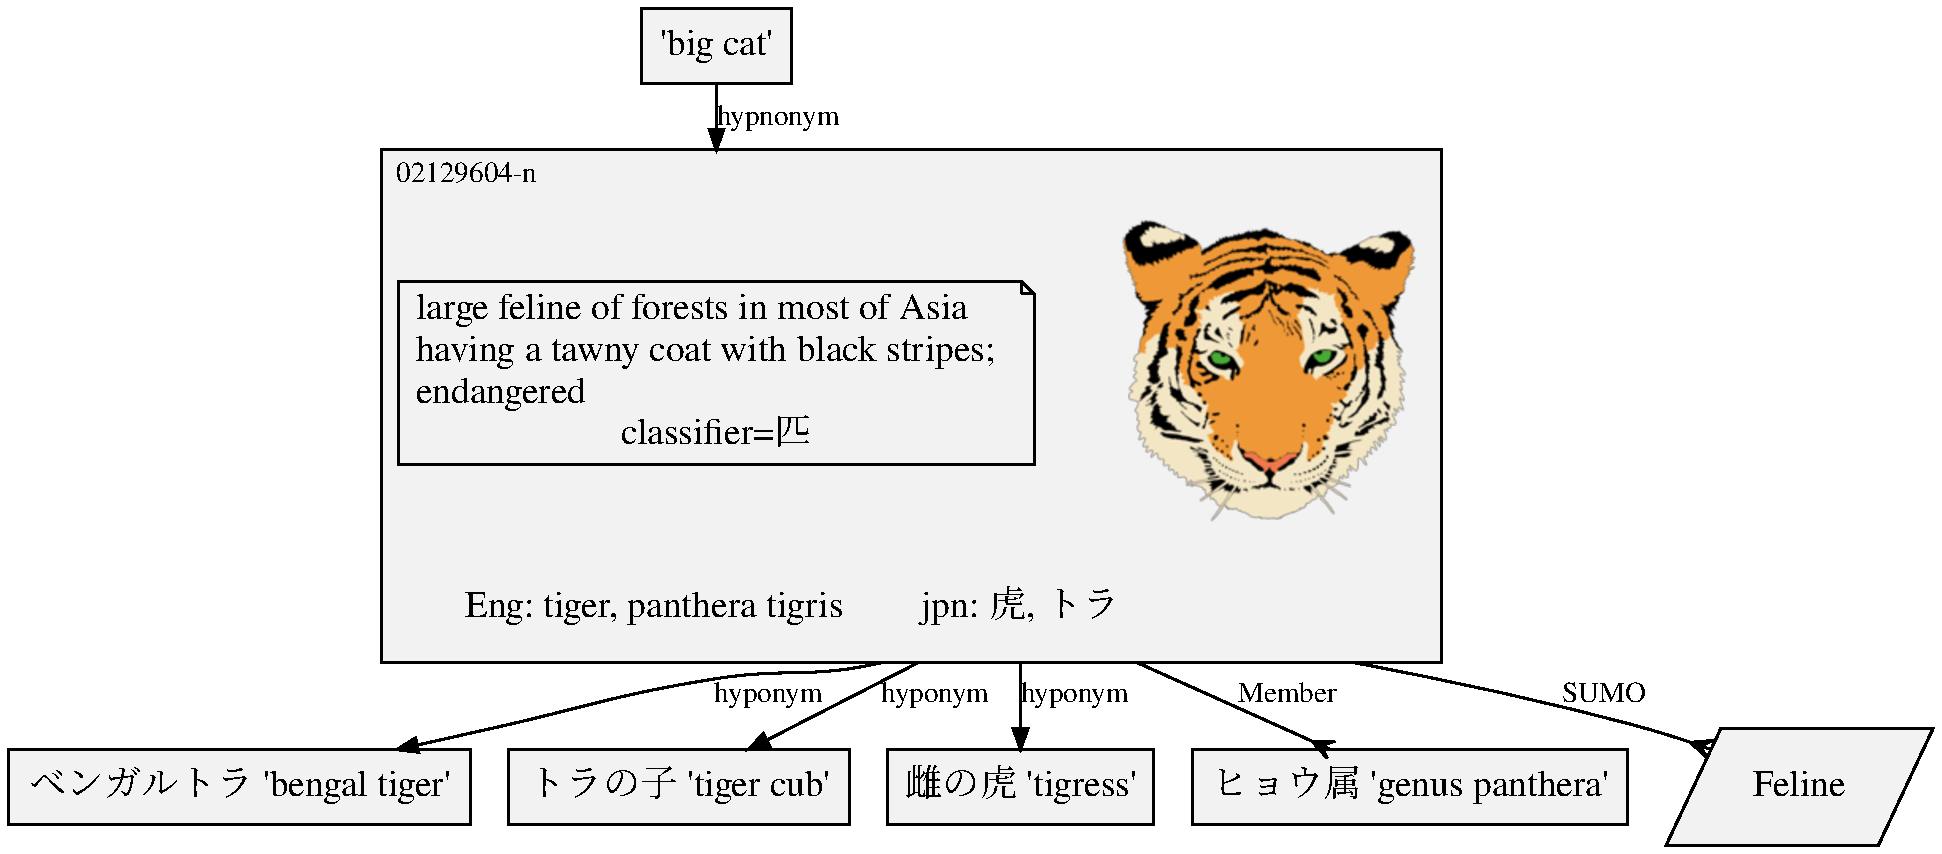
\includegraphics[width=0.9\textwidth]{img/wn-jpn-tiger.pdf}

Here we show English and Japanese.
\end{frame}

\begin{frame}{Another view of \eng{cat} as a graph}
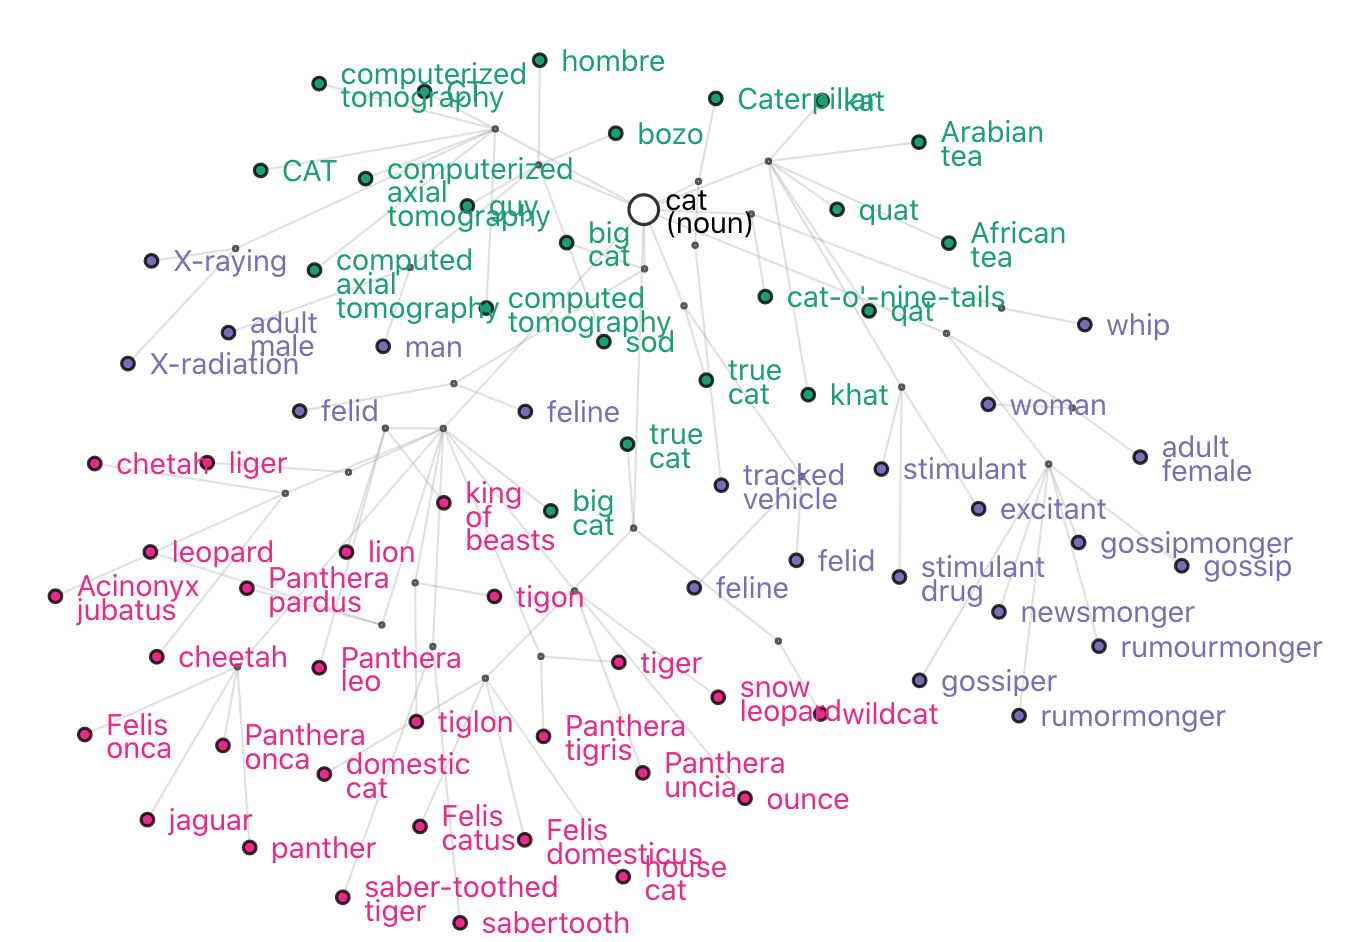
\includegraphics[width=0.9\textwidth]{img/graph.png}

From \url{https://github.com/aliiae/lexical-graph}
\end{frame}

\begin{frame}{Many people wanted to have wordnets}

  \begin{itemize}
   \item \textbf{EuroWordNet} \citep{_Vossen:1998}:  
  Dutch, English, German, French, Spanish, Italian

  \item \textbf{BalkaNet}:  
  Bulgarian, Greek, Romanian, Serbian, Turkish

  \item \textbf{Asian WordNet}:  
  Japanese, Korean, Thai, Indonesian, Vietnamese, Mongolian, Burmese

  \item \textbf{IndoWordNet}:  
  Hindi, Bengali, Marathi, Gujarati, Punjabi, Urdu, Tamil, Telugu, Kannada, Malayalam, Odia, Assamese, Nepali, Konkani, Manipuri, Kashmiri, Sanskrit
\end{itemize}

And many individual projects not listed here.

\end{frame}



    
\subsection{Wordnets in the World}

\begin{frame}{Wordnets in the world 2008-06}
 Many wordnets, but few free: we wanted to build an open wordnet for Japanese and needed other wordnets for cross-lingual disambiguation.
 \begin{center}
   \noindent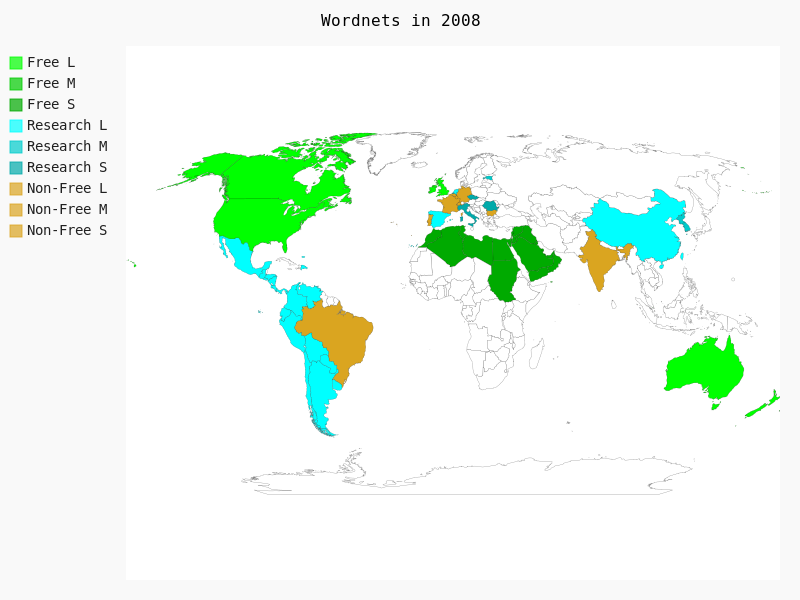
\includegraphics[width=1.0\textwidth]{img/wns-2008.png}
 \end{center}
Green is free; Blue is research only; Brown costs money

\end{frame}


\begin{frame}{Wordnets in the world 2008-06}

  \begin{itemize}
  \item When we decided to build the Japanese wordnet, we wanted to
    leverage existing work and use multiple languages to disambiguate
  \item Many wordnets existed, but few were free and almost all came
    in slightly (or radically) different formats.
    \begin{itemize}
    \item PWN had a loop!
    \item GWG grid had bad encodings
    \item There was \emp{no} wordnet that worked out of the box
    \item  Different projects even used different names for pos
      \\ e.g., Adjective ($a$ vs $j$); Adverb ($r$ vs $b$) 
    \end{itemize}
  \item There was no easy shared access
  \item We had to massage the data for our project
  \item  We wanted to try to save other people the trouble we
    experienced, and make the normalized data available (where legally possible)
  \end{itemize}
\end{frame}




\begin{frame}{Wordnets in the world 2011-06}
Free wordnets for French, Catalan, Polish, Thai and \txx{Japanese}
\begin{center}
  \noindent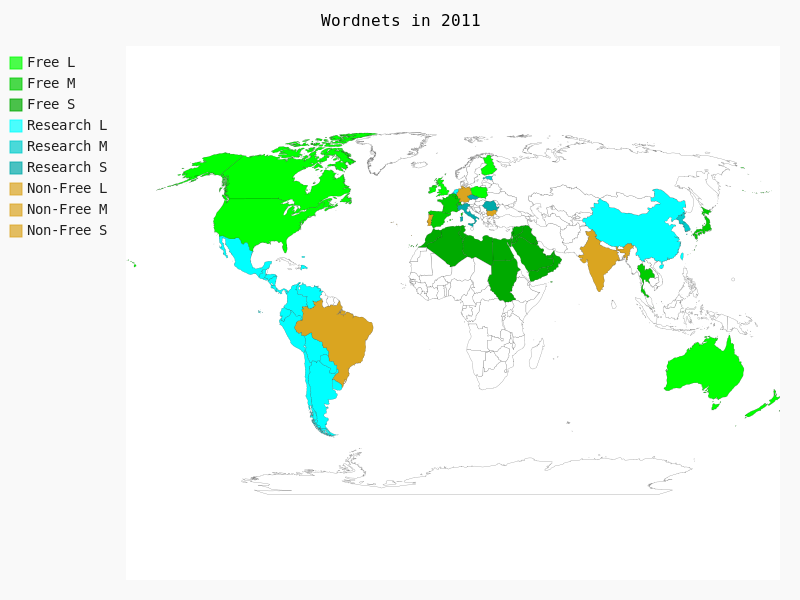
\includegraphics[width=1.0\textwidth]{img/wns-2011.png}
\end{center}
Green is free; Blue is research only; Brown costs money
\end{frame}


\begin{frame}{Wordnets in the world 2012-06}
Spanish freed (and Galician and Basque), Farsi, Norwegian, Swedish, \txx{Bahasa} (Malay and Indonesian)
\begin{center}
  \noindent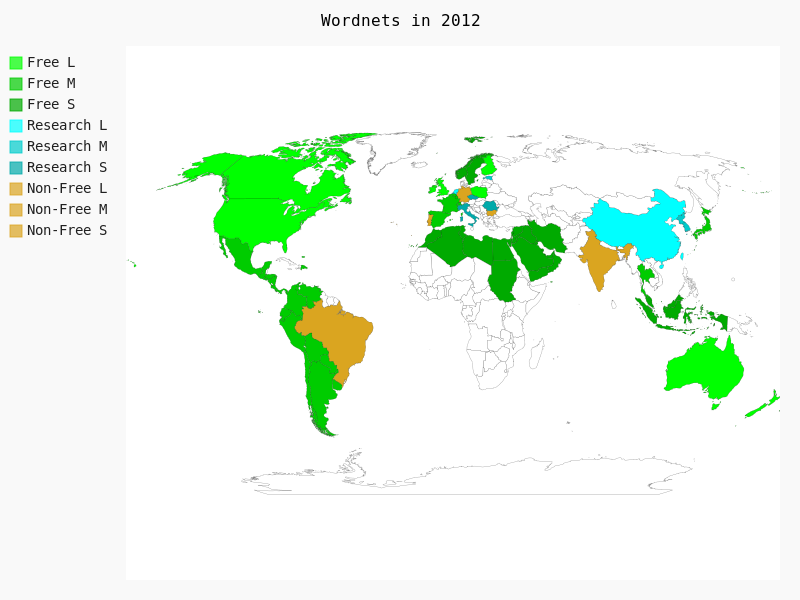
\includegraphics[width=1.0\textwidth]{img/wns-2012.png}
\end{center}
Green is free; Blue is research only; Brown costs money
\end{frame}

\begin{frame}{Wordnets in the world 2013-06}
\txx{Chinese} Open Wordnet (and Chinese wordnet)
\begin{center}
  \noindent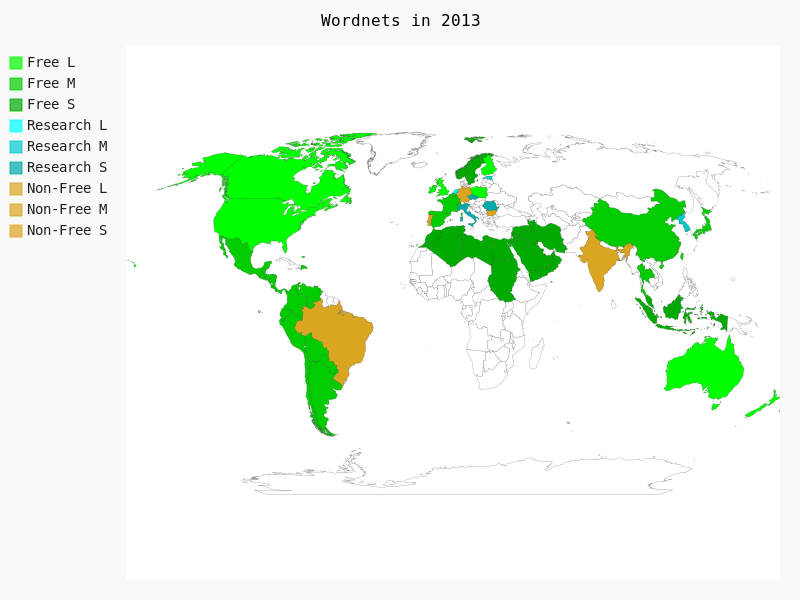
\includegraphics[width=1.0\textwidth]{img/wns-2013.png}
\end{center}
Green is free; Blue is research only; Brown costs money
\end{frame}


% \begin{frame}{Wordnets in the world 2014-06}
% Swedish
% \begin{center}
%   \noindent\includegraphics[width=1.0\textwidth]{WordNet-map-2014-06}
% \end{center}
% Green is free; Blue is research only; Brown costs money
% \end{frame}



% \begin{frame}{Wordnets in the world 2015-06}

% \begin{center}
%   \noindent\includegraphics[width=1.0\textwidth]{WordNet-map-2015-06}
% \end{center}
% Green is free; Blue is research only; Brown costs money
% %\MyLogo{}
% %\MyLogo{}
% \end{frame}



\begin{frame}{Wordnets in the world 2016-01}
Swedish, Dutch, Icelandic, Lithuanian, Romanian, \ldots
\begin{center}
  \noindent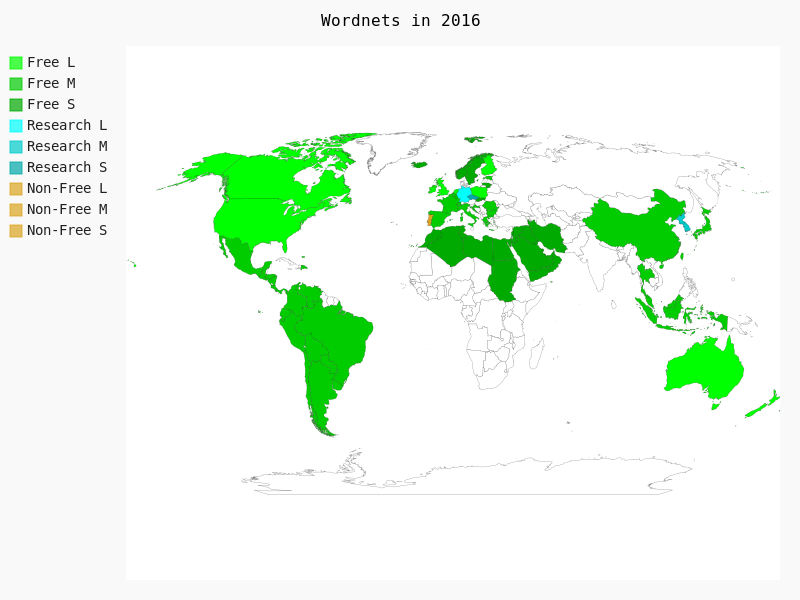
\includegraphics[width=1.0\textwidth]{img/wns-2016.png}
\end{center}
Green is free; Blue is research only; Brown costs money
%\MyLogo{}
%\MyLogo{}
\end{frame}



\begin{frame}{}
\frametitle{Why do we want so many?}
\begin{itemize}
\item Every new wordnet makes the network much richer $n(n-1)$ lexicons!
\item Multilingual disambiguation makes it easier to add new languages
\item New languages add new phenomena 
  \begin{itemize}
  \item and new synsets/concepts
  \item and new relations
  \end{itemize}
\item More users mean more bugs found
\item New approaches can be shared
  \begin{itemize}
  \item UKB  (does graph-based WSD) \hfill Basque
  \item Wordnet glosses  (disambiguates wordnet definitions) \hfill Princeton 
  \item Logical forms  (gives LF for wordnet definitions) \hfill USC/ISI
  \item UKB + Wordnet glosses + Logical forms  (better WSD) \hfill Bulgaria
  \item[\ldots]
  \end{itemize}
\end{itemize}
\end{frame}

\begin{frame}{How did we open the data?}
  \begin{itemize}
  \item Leading by example (we made open wordnets for Japanese, Bahasa, Chinese)
  \item Appeal to self-interest: we showed that open resources are cited more
     \citep{Bond:Paik:2012}
  \item Simple format for sharing (tsv) --- I wrote many converters
    \\ Many checks for ill-formed lexicons
  \item Public praise for freed resources
  \item Private persuasion for non-open resources
  \item Open website 
    \begin{itemize}
    \item online interface (with statistics on coverage)
    \item downloadable in multiple formats
    \item linked to other resources (sentiment, time, SUMO, \ldots)
    \end{itemize}
  \item Used by other projects: Google Translate; 
    Natural Language Toolkit (NLTK); Babelnet
  \end{itemize}
\end{frame}


\begin{frame}{Wordnets in the world 2017-12}
Added: Moroccan Arabic, Abui, Myanmar, Sesotho, Tswana, Venda, Xhosa, Zulu;
\\Ancient: Greek, Latin, Sanskrit;
\\ Freed: German, Estonian, Romanian, Czech
\begin{center}
  \noindent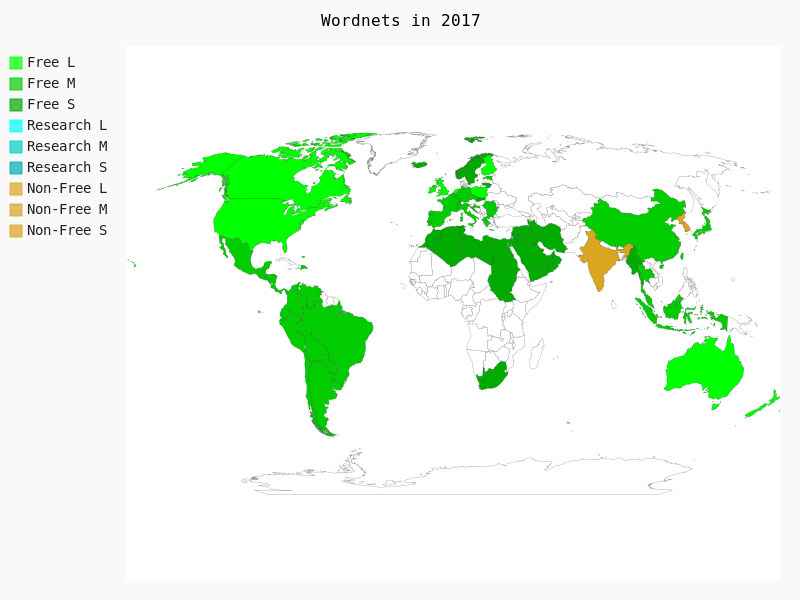
\includegraphics[width=1.0\textwidth]{img/wns-2017.png}
\end{center}
%Green is free; Blue is research only; Brown costs money
%\MyLogo{}
%\MyLogo{}
\end{frame}

\begin{frame}{Wordnets in the world 2019-06}
  Added: Cantonese, Coptic, Russian, Mongolian, Danish
  \\ Expanded: English
\begin{center}
  \noindent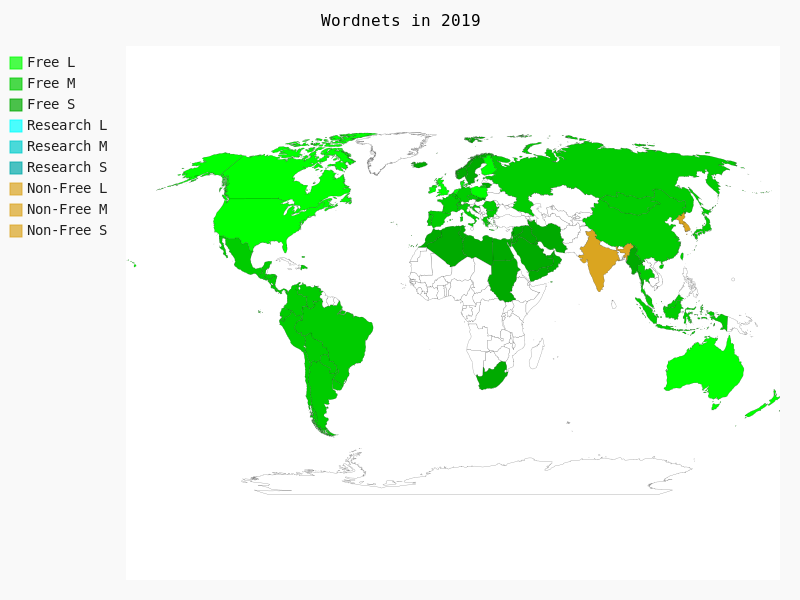
\includegraphics[width=1.0\textwidth]{img/wns-2019.png}
\end{center}
\end{frame}

\begin{frame}{Wordnets in the world 2021-01}
  Added: Uzbek, Turkish;
\\  Richer inventory of relations, better documentation
\begin{center}
  \noindent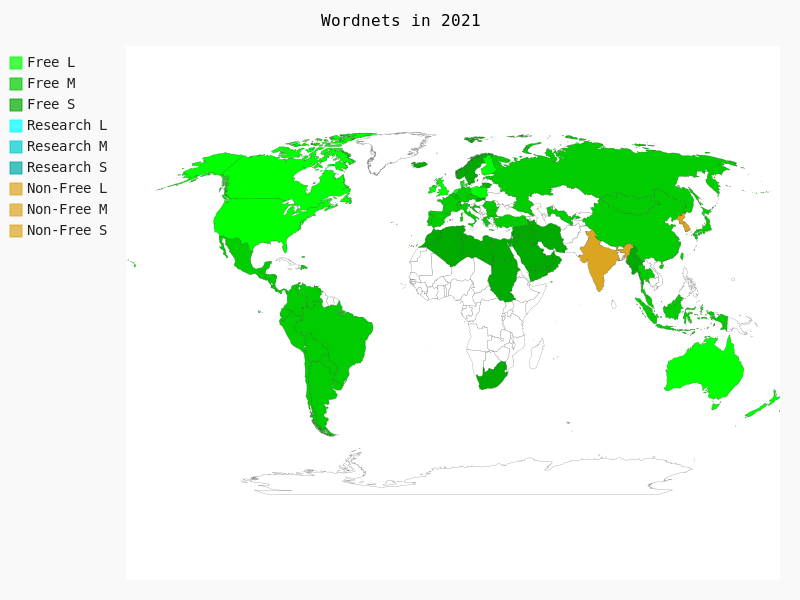
\includegraphics[width=1.0\textwidth]{img/wns-2021.png}
\end{center}
\end{frame}

\begin{frame}{Wordnets in the world 2023-01}
  Added: Ukrainian;
\\  Richer inventory of relations, better documentation
\begin{center}
  \noindent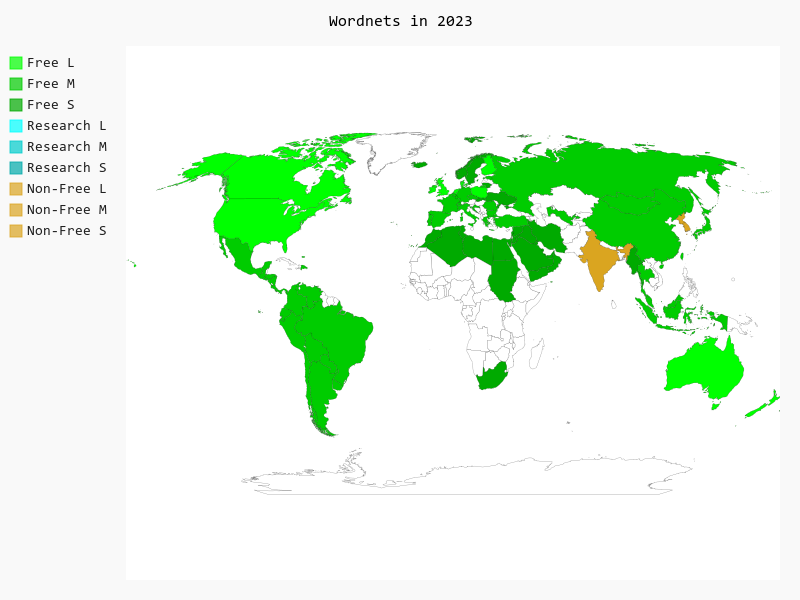
\includegraphics[width=1.0\textwidth]{img/wns-2023.png}
\end{center}
\end{frame}



\begin{frame}{Current state}
  \begin{itemize}
  \item 120,000+ synsets from the Open English Wordnet
    \begin{itemize}
    \item 2,000 added locally 
    \end{itemize}
  \item 35 curated wordnets with 2,000,000 senses
  \item 250 languages with automatically created senses from
    wiktionary (at least 100 senses per language)
  \item 1,200 languages with senses mapped from various Swadesh lists
    (around 100-200 senses/language)
  \end{itemize}
\end{frame}



% \begin{frame}{Open Wordnets in the world 2017-01}


%   \begin{large}
%     Albanet; Arabic WordNet (AWN v2); BulTreeBank Wordnet (BTB-WN);
%     Chinese Open Wordnet; Chinese Wordnet (Taiwan); DanNet; Greek
%     Wordnet; Princeton WordNet; Persian Wordnet; FinnWordNet; WOLF
%     (Wordnet Libre du Français); Hebrew Wordnet; Croatian Wordnet;
%     IceWordNet; MultiWordNet; ItalWordnet; Japanese Wordnet;
%     Multilingual Central Repository (Spanish, Galician, Catalan,
%     Basque); Wordnet Bahasa (Malay, Indonesian); Open
%     Dutch WordNet; Norwegian Wordnet (Bokmal); Norwegian Wordnet
%     (Nynorsk); plWordNet; OpenWN-PT; Romanian Wordnet; Lithuanian
%     WordNet; Slovak WordNet; sloWNet; Swedish (SALDO); Thai Wordnet
%   \end{large}
        \nocite{Ruci:2008,Black:Elkateb:Rodriguez:Alkhalifa:Vossen:Pease:Bertran:Fellbaum:2006,Borin:Forsberg:Lonngren:2013,Pedersen:2009,Simov:Osenova:2010,Gonzalez-Agirre:Laparra:Rigau:2012,Pociello:Agirre:Aldezabal:2011,Wang:Bond:2013,Huang:Hsieh:Hong:Chen:Su:Chen:Huang:2010,Pedersen:2009,_Fellbaum:1998,Stamou:Nenadic:Christodoulakis:2004,Sagot:Fiser:2008,Ordan:Wintner:2007,Noor:Sapuan:Bond:2011,Isahara:Bond:Uchimoto:Utiyama:Kanzaki:2008,Montazery:Faili:2010,Linden:Carlson:2010,Garabik:Pileckyte:2013,Vossen:Postma:2014,Piasecki:Szpakowicz:Broda:2009,Paiva:Rademaker:Melo:2012,Tufis:Ion:Bozianu:Ceausu:Stefanescu:2008,Fiser:Novak:Eejavec:2012,Borin:Forsberg:Lonngren:2013,Thoongsup:Charoenporn:Robkop:Sinthurahat:Mokarat:Sornlertlamvanich:Isahara:2009,Pianta:Bentivogli:Girardi:2002,Oliver:Sojat:Srebacic:2015,Raffaelli:2008,Toral:Bracal:Monachini:Sora:2010}

        
% \medskip
% And in the pipeline: Irish, Ancient Greek, Latin, Myanmar, Abui, \ldots
%\end{frame}

\begin{frame}{}
\frametitle{The Open Multilingual Wordnet 1.0}
\begin{itemize}
\item Defined a minimal shared format (incrementally useful)
  \\ based on the hierarchy of PWN~3.0 (most wordnets are translations)
  \begin{itemize}
  \item \txx{name, license, URL} (metadata)
  \item \txx{synset \& lemma} pairs (linked to PWN)
  \item later also \txx{definitions} and \txx{examples} 
  \end{itemize}
\item Wrote conversion scripts to extract this information
  \begin{itemize}
  \item Provided feedback when there were errors
  \item Occasionally suggested improvements
  \end{itemize}
\item Encouraged people to choose an open license 
  \\ we are deriving a   new resource and redistributing 
  \\ --- this needs permission
\item Linked each resource to its canonical citation
  \\ Encouraged people to cite the papers when they used the wordnets
\end{itemize}
Mostly done by me on weekends, some help from Lars Nygaard, John McCrae and of course the individual projects.
\end{frame}

\begin{frame}{What else did we do?}
  \begin{itemize}
  \item Minimal evaluation
    \begin{itemize}
    \item Coverage of core concepts
      \\ made the core concept list more easily available
    \end{itemize}
  \item Created a common search interface
    \begin{itemize}
    \item with links to other external resources: SUMO, sentiment, temporal, \ldots
    \end{itemize}
  \item Provided downloads in standard formats (LMF, LEMON)
  \item Automatically created wordnets from Wiktionary and CLDR
    \begin{itemize}
    \item shared this data freely 
    \end{itemize}
  \item Created a Python API to access the data in NLTK \citep{Bird:Klein:Loper:2009}
    \begin{itemize}
    \item Extended the NLTK corpus class to add information about recommended citation and licenses (for all corpora, not just the wordnets)
    \item New wordnets and updates are still being added
    \end{itemize}
  \end{itemize}

\end{frame}



% \subsection{NLTK}


% \begin{frame}[fragile]{Python API: NLTK}

% \begin{verbatim}
% >> import nltk
% >>> from nltk.corpus import wordnet as wn
% >>> wn.synsets('dog')
%  [Synset('dog.n.01'), Synset('frump.n.01'), 
%   Synset('dog.n.03'), Synset('cad.n.01'), 
%   Synset('frank.n.02'),  Synset('pawl.n.01'), 
%   Synset('andiron.n.01'), Synset('chase.v.01')]

% >>> wn.synsets('dog')[0].definition()
%  'a member of the genus Canis (probably descended 
%   from the common wolf) that has been domesticated 
%   by man since prehistoric times; occurs in many breeds'
% \end{verbatim}
% \end{frame}

% \begin{frame}[fragile]{Python API: NLTK}

% \begin{verbatim}
% >>> wn.synsets('dog')[0].lemmas(lang='jpn')
%  [Lemma('dog.n.01.イヌ'), Lemma('dog.n.01.ドッグ'), 
%   Lemma('dog.n.01.洋犬'), Lemma('dog.n.01.犬')]

% >>> wn.synsets('dog')[0].lemmas(lang='zsm')
%  [Lemma('dog.n.01.anjing')]

% >>> wn.synsets('dog')[0].hypernym_paths()[0]
%  [Synset('entity.n.01'), Synset('physical_entity.n.01'), 
%   Synset('object.n.01'), Synset('whole.n.02'), 
%   Synset('living_thing.n.01'), Synset('organism.n.01'), 
%   Synset('animal.n.01'), Synset('chordate.n.01'), 
%   Synset('vertebrate.n.01'), Synset('mammal.n.01'), 
%   Synset('placental.n.01'), Synset('carnivore.n.01'), 
%   Synset('canine.n.02'), Synset('dog.n.01')]
% \end{verbatim}
% \end{frame}




% \subsection{Chinese Open Wordnet}
% \begin{frame}{Chinese Open Wordnet (COW)}

%   \begin{itemize}
%   \item \href{http://compling.hss.ntu.edu.sg/cow/}{Chinese Open
%       Wordnet --- 汉语开放词网
% }
%   \item 42,315 synsets
%   \item 79,812 senses
%   \item 61,536 unique words
%   \item built by Shan Wang and Francis Bond
%     \begin{itemize}
%     \item with cooperation from Chinese Wordnet (South Eastern
%       University), Bilingual Ontological Wordnet (Academica Sinica) and OMW
%     \end{itemize}
%   \item new release coming soon with pronouns, exclamatives,
%     classifiers, chengyu and pinyin.
%   \item We would like more collaborators, \ldots
%   \end{itemize}

% \end{frame}


% \begin{frame}{Chengyu}
%   \begin{itemize}
%   \item include pinyin for entries, with multiple variants
%     \begin{itemize}
%     \item \cmn[woman]{女人}
%     \item \cmn{nǚrén}
%     \item \cmn{nü3ren2}
%     \item \cmn{nv3ren2}
%     \item \cmn{nüren}
%     \item \cmn{nvren}
%     \end{itemize}
%   \item pinyin added from open source lexicons, with a confidence
%     based on whether we found the whole word and if it was ambiguous
%     or not
%   \end{itemize}

% \end{frame}

% \begin{frame}{Interjections}
%   \begin{avm}
% \[ \wnida{\wnid{80000000-x} (pain)}
% eng-lemmas & \parbox[t]{0.6\textwidth}{\eng{ah, oh, ouch, ow, wow, yipe, yow}} \\ 
% cmn-lemmas & \parbox[t]{0.6\textwidth}{\cmn{哎呀, 啊呀, 哎哟, 啊哟, 哎哟喂, 疼}} \\ 
% definition & \parbox[t]{0.6\textwidth}{an expression that is uttered to show physical hurt or pain} \\ 
% exemplifies & \wnid{15167474-n} (utterance) \\ 
% see also & \wnid{14322699-n} (pain, hurting) \]
% \end{avm} \\
% \begin{avm}
% \[ \wnida{\wnid{80000002-x} (checkmate)}
% eng-lemmas & \eng{checkmate, mate}  \\ 
% cmn-lemmas & \eng{将死}  \\ 
% definition & \parbox[t]{0.6\textwidth}{an expression that is uttered during a game of chess to declare that the final winning move has taken place} \\ 
% exemplifies & \wnid{15167474-n} (utterance) \\ 
% see also & \wnid{00167764-n} (checkmate) \]
% \end{avm}
% \end{frame}

% \begin{frame}{Classifiers}
%   \begin{small}
% \begin{avm}
% \[ \wnida{80000003-x }
% cmn-lemmas & \textcolor{teal}{把} \cmn{bǎ} \\ 
% \parbox[t]{0.2\textwidth}{definition} & \parbox[t]{0.6\textwidth}{a sortal classifier used with tools and objects with a handle, such as hammers, brooms, guitars or teapots} \\ 
% exemplifies & \wnid{06308436-n} (classifier) \\
% classifies & \wnid{03481172-n} (hammer) \\
% classifies & \wnid{02906734-n} (broom) \\
% classifies & \wnid{04398044-n} (teapot) \]
% \end{avm} \\

% % \begin{avm}
% % \[ \wnida{80000004-x }
% % lemmas & \textcolor{teal}{根} \jpn{gen} \\ 
% % definition & \parbox[t]{16em}{a sortal classifier used for long slender objects, such as a banana, a pillar, a sausage or a needle} \\ 
% % domain usage & \wnid{06308436-n} (classifier)  \]
% % \end{avm} \\

% \begin{avm}
% \[ \wnida{80000004-x }
% jpn-lemmas & \textcolor{teal}{振} \jpn{furi} \\ 
% \parbox[t]{0.2\textwidth}{definition} & \parbox[t]{0.6\textwidth}{a sortal classifier used for weapons with a blade, such as knifes, swords or daggers} \\ 
% exemplifies & \wnid{06308436-n} (classifier) \\
% classifies & \wnid{03624134-n} (knife) \\
% classifies & \wnid{04373894-n} (sword) \\
% classifies & \wnid{03158885-n} (dagger) \]
% \end{avm}
    
%   \end{small}
% \end{frame}

% \begin{frame}{Idioms}
%   \begin{avm}
%     \[ \wnida{80000005-a}
% cmn-lemmas & \textcolor{teal}{根深蒂固} \cmn{gēnshēndìgù} \\ 
% \parbox[t]{0.2\textwidth}{definition$_{eng}$}
% & \parbox[t]{0.6\textwidth}{deep-rooted (lit: roots deep stem strong)}
% \\ 
% \parbox[t]{0.2\textwidth}{definition$_{cmn}$} & \parbox[t]{0.6\textwidth}{基础深厚，难以动摇} \\ 
% exemplifies & \wn{chengyu}{n}{1}  \\
% similar-to  & \wn{deep-rooted}{a}{1} \\
%  example & \[ essay$_{176}$ & 罪魁祸首自然是那些\wemp{根深蒂固}的\\
%                    &  错误和持续的恶性循环。 \\
%                     news$_{101303}$ & 另外，对再次被日本统治的警戒 \\
%                    &   论也\wemp{根深蒂固}。 \\
%                     news$_{101421}$ & 对贝鲁斯柯尼的搜查是成为促使 \\
%                    &  这个战后政治崩溃之契机的净化 \\
%                    &  作战的一环，问题\wemp{根深蒂固}。\] \\
%        xref & \[ Chengyu500 & \#37 p122  \]
% \]
%   \end{avm}
% \end{frame}
\subsection{The Japanese Wordnet}

\begin{frame}{The Japanese Wordnet}
\begin{itemize}
\item Initially assume that the semantic structure is the same
  \begin{itemize}
  \item \lex{dog} $\subset$ \eng{animal}
  \item[$\Rightarrow$] \lex{\ja{犬}} $\subset$ \lex{\ja{動物}}
  \end{itemize}
\item Added Japanese words to Princeton wordnet synsets
\end{itemize}
\begin{tabular}{ccrrrl}
  Date       & Ver & Concepts & Words & Senses  & Misc \\ \hline
  2009-02-28 & 0.90 &  49,190 & 75,966 & 156,684 & initial release \\
  2009-08-31 & 0.91 &  50,739 & 88,146 & 151,831 & linked to SUMO \\
  2009-11-16 & 0.91 &  49,655 & 87,133 & 146,811  & \\
  2010-03-05 & 1.00 &  56,741 & 92,241 & 157,398 & + definitions, examples \\
  2010-10-22 & 1.10 &  57,238 & 93,834 & 158,058 & \\
  2012-01-06 &      &         &        &          & Japanese Semcor \\
  2014-02-06 &      &         &        &          & NLTK module \\
  \textbf{2022-05-22} & 2.0  &  58,039 & 89,902 & 147,207 & 386,222  variants \\
\end{tabular}
\end{frame}

\begin{frame}{Japanese Wordnet 2.0}
  \begin{itemize}
  \item This release uses a new format (GWA XML 1.0)
    \begin{itemize}
    \item Allows for variant forms
    \item Structure can be different from PWN
      \begin{itemize}
      \item 788 new concepts (synsets)
      \end{itemize}
    \item Includes frequencies from JSemCor and NTU-MC
    \end{itemize}
  \item A long slog by Takayuki Kuribayashi to add the forms
    
  \end{itemize}
\end{frame}


\begin{frame}{Orthographic Variants}

  {\jafont
  \begin{itemize}
  \item synsetID=14728724-n (Eng: protein)
    \\ プロテイン, 蛋白質, タンパク, たんぱく質, 蛋白, タンパク\,質
    \\ \hspace{15em} ↓
    \\ \textbf{蛋白質} (\,タンパクシツ, たんぱ\,質, タンパク\,質, たんぱくしつ)
    \\ \textbf{蛋白} (タンパク, たんぱく)
    \\ \textbf{プロティン} (プロテイン, ぷろてぃん)
  \item synsetID=02765464-v (Eng: absorb, take in)
    \\ 呑みこむ, 呑\,込む, 吸引, 吸い\,込む, 吸収
    \\\hspace{20em} ↓
    \\ \textbf{吸い込む}  (\,スイコム, 吸\,込む, 吸いこむ, すいこむ)
    \\ \textbf{吸収} (キュウシュウ, きゅうしゅう)
    \\ \textbf{吸引} キュウイン, きゅういん)
    \\ \textbf{飲み\,込む} (ノミコム, 飲\,込む, 呑み\,込む, 呑\,込む, 呑みこむ, のみ\,込む, のみこむ
  \end{itemize}}
\end{frame}

\begin{frame}{Other extensions}
  \begin{itemize}
  \item Added pronouns and demonstratives
    \\ \lex{\ja{私, この, その, あの, どの}}
  \item Added classifiers
    \\ \lex{\ja{人, 台, 匹, 回}}
  \item Added 4-character idioms
    \\ \lex{\ja{五十歩百歩}}
  \item Added corpus-based examples and sense frequency
    \\ \lex{\ja{対策}}$_3$, \lex{\ja{策}}$_3$, \lex{\ja{措置}}$_2$, \lex{\ja{方略, 方策, 術, 打つ手}}
    ``step, measure''
   \item Added exclamatives
    \\ \lex{\ja{王手, ヨイショ, お\,早うございます}}
  \end{itemize}
\end{frame}


\begin{frame}{Ontological Differences: Temperature}

  \begin{itemize}
  \item English uses the same words for temperature experienced by
    touching or as a general feeling:
\\ \horn{cold, cool, warm, hot}
\item Japanese distinguishes
  \begin{itemize}
  \item the feeling: \horn{\ja{寒い, 涼しい, 温かい, 暑い}}
  \item to-touch:  \horn{\scalebox{2}[1]{\ja{冷い}}, \ja{暖か, 熱い}}
  \end{itemize}
\item English uses a single word for water of any temperature:
  \lex{water}
\item Japanese uses different words for cold (non-hot) water and hot
  water: \lex{\ja{水}} vs \lex{\ja{湯}}
\item We are doing our best to add native Japanese concepts, even if not lexicalized in English
\end{itemize}

It raised an interesting question about interlingal equivalence ---
should \lex{water} link to \lex{\ja{水}} or do we need a non lexicalized entry \lex{\ja{水}}-or-\lex{\ja{湯}}?  

\end{frame}

\begin{frame}{Hierarchy}
  \begin{center}
  \begin{forest}
 [ temperature 
   [ cold, name=cold
      [ \ja{寒い}, name=cold1 ]
      [ \ja{冷たい}, name=cold2 ]
      ]
    [ cool, name=cool
      [ \ja{涼しい}, name=cool1 ]
    ]
      [ warm, name=warm
      [ \ja{暖かい}, name=warm1 ]
      [ \ja{温かい}, name=warm2 ]
     ]
   [hot, name=hot
    [ \ja{暑い}, name=hot1 ]
    [ \ja{熱い}, name=hot2 ]
   ]
   ]
   \draw [dashed,to-to](cold.east) to[out=-15,in=-165]  (hot.west);
   \draw [dashed,to-to](cool.east) to[out=-15,in=-165]  (warm.west);
   \draw [dashed,to-to](cold1.south) to[out=-30,in=-150]  (hot1.south);
   \draw [dashed,to-to](cold2.south) to[out=-30,in=-150]  (hot2.south);
    \draw [dashed,to-to](cool1.south) to[out=-15,in=-165]  (warm1.south);
  \end{forest}
\end{center}

\begin{itemize}
\item Some nodes are not lexicalized in Japanese, but still useful for the structure
\item \txx{temperature} is linked by \lnk{attribute} (\ja{属性}); tree is \lnk{hyponym} 
  \\ dashed arrows are \lnk{antonym}
  
\end{itemize}

\end{frame}

\begin{frame}{Ontological Differences: Kin}
  \begin{tikzpicture}
\tikzset{level distance=12ex}
\Tree [.\node(ja){\begin{avm}% 
    \[ \wnida{jwn:3478-n}
    lemma & \eng{\ja{姉妹兄弟, 兄弟}} \\
    \]\end{avm}};
      [.\node(jb){\begin{avm}% 
    \[ \wnida{jwn:6597-n}
    lemma & \eng{\ja{兄弟, 男兄弟}} \\
    \]\end{avm}}; 
 [.\node(je){\begin{avm}% 
    \[ \wnida{jwn:6897-n}
    lemma & \eng{\ja{兄}} \\
    \]\end{avm}}; ]
 [.\node(jf){\begin{avm}% 
    \[ \wnida{jwn:5957-n}
    lemma & \eng{\ja{弟}} \\
    \]\end{avm}}; ]
]
      [.\node(jc){\begin{avm}% 
    \[ \wnida{jwn:8745-n}
    lemma & \eng{\ja{姉妹}} \\
    \]\end{avm}};  [.\node(jg){\begin{avm}% 
    \[ \wnida{jwn:2897-n}
    lemma & \eng{\ja{姉}} \\
    \]\end{avm}}; ]
 [.\node(jh){\begin{avm}% 
    \[ \wnida{jwn:2957-n}
    lemma & \eng{\ja{妹}} \\
    \]\end{avm}}; ]]
         ]
    \end{tikzpicture}

    \begin{itemize}
    \item More accurately models Japanese
    \item We aim to cover at least the TUFS basic vocabulary
    \end{itemize}


  
\end{frame}
\begin{frame}[allowframebreaks]{Other Examples --- \ja{ロングテール} ``long tail''}
  \begin{exe}
  \ex \label{wn:soba}
\begin{avm} \small
\[ \wnida{\wnid{80001626-n} (soba\_noodle)}
lemmas:jpn &\wnbox{\ja{蕎麦}} \\
lemmas:eng &\wnbox{soba} \\
def:jpn &\wnbox{\ja{そば\,粉で\,作られた\,細い\,麺}} \\
def:eng &\wnbox{narrow noodle made from buckwheat}\\
hypernym &  (noodle) \\ 
\]
\end{avm}
\ex \label{wn:hajjah}
\begin{avm} \small
\[ \wnida{\wnid{80002377-n} (castle construction)}
  lemmas:jpn &\wnbox{\ja{築城} \jpn{chikujou}} \\
def:jpn &\wnbox{\ja{城の\,建設}} \\
def:eng &\wnbox{the construction of castles}\\
hypernym &  (construction) \\ 
\]
\end{avm}
\newpage


\ex \label{wn:student}
\begin{avm} \small
\[ \wnida{\wnid{90000315-n} (hajjah)}
  lemmas:jpn &\wnbox{\ja{ハジャ}} \\
lemmas:eng &\wnbox{hajjah} \\
  def:jpn &\wnbox{\ja{メッカへの\,巡礼を\,行った\,女性}} \\
def:eng &\wnbox{a woman who has made the pilgrimage to Mecca}\\
hypernym &  (haji) \\
category & (muslim)
\]
\end{avm}

\ex
\begin{avm} \small
\[ \wnida{\wnid{80001731-n} (exchange student)}
  lemmas:jpn &\wnbox{\ja{留学生}} \\
lemmas:eng &\wnbox{exchange student} \\
  def:jpn &\wnbox{\ja{海外で\,勉強する\,学生}} \\
def:eng &\wnbox{a student who studies abroad}\\
hypernym &  (student) \\
\]
\end{avm}

\ex \label{wn:shunto}
\begin{avm} \small
\[ \wnida{\wnid{80000338-n} (Shunto)}
  lemmas:jpn &\wnbox{\ja{春闘}} \\
  lemmas:eng &\wnbox{spring wage negotiation, spring wage offensive, Shunto} \\
  def:jpn &\wnbox{\ja{毎年労働組合が、賃金引き\,上げなどの}} \\
   &\wnbox{\ja{\ \ \ \  要求を\,掲げて\,行う\,全国的な\,闘争}} \\
def:eng &\wnbox{annual event by Japanese workers unions when wages are renegotiated}\\
hypernym &  (protest) \\ 
\]
\end{avm}
 

\end{exe}

\end{frame}


% \subsection{Korean Wordnets}
% \begin{frame}{Korean Wordnets}

%   \begin{itemize}
%   \item There is a good wordnet built at Pusan National University
%     \citep{Yoon:Hwang:Lee:Kwon:2009}, but unfortunately it is not open
%   \item There is a small wordnet built from the Tokyo University of
%     Foreign Studies Basic Vocabulary list
%     \begin{itemize}
%     \item It is free (CC By 4.0)
%     \item 527 concepts; 1,011 words; 1,698 example sentences
%       \begin{avm}
%         \[ \wnida{10694258-n}
%           en-lemmas & \cmn{teacher} \\
%           ko-lemmas & \textcolor{teal}{선생님} \cmn{seonsaengnim} \\ 
%           \parbox[t]{0.2\textwidth}{definition} & \parbox[t]{0.6\textwidth}{a person whose occupation is teaching} \\
%           ko-example & \ul{선생님}, 이 보고서 말인데요, 마감이 내일까지죠?
%           \]
%         \end{avm} 
%       \item Not really big enough to do much with
%       \item and biased to teaching --- should the entry be just 선생?
%     \end{itemize}
    
%   \end{itemize}
% \end{frame}

\subsection{The Open English Wordnet}
  \begin{frame}{The Open English Wordnet}
      \begin{itemize}
      \item The successor to the Princeton Wordnet (which is no
        longer developed)
      \item New vocabulary (thousands of new words and senses)
      \item New relationships (\lnk{taboo}, \lnk{agent}, \lnk{female-form})
      \item Many, many bug fixes
      \item Pronunciation (in IPA)
      \end{itemize}

  \end{frame}

  
% \begin{frame}{Open Multilingual Wordnet 2.0}

%   \begin{itemize}
%   \item Instead of a single hierarchy (PWN~3.0) it is the union of
%     multiple hierarchies
%     \begin{itemize}
%     \item Allow links (relations) and nodes (synsets) not in PWN
%       \begin{itemize}
%       \item Merge nodes that link to the same Interlingual Index
%         record
%       \item Map all semantic relations to a known subset
%       \item Document them
%       \item Add more as the need is shown
%       \end{itemize}
%       \item Now we can better add in differently structured wordnets
%         like Polish, Dutch or Gaelic
%     \end{itemize}
%   \item The goal is to have a useful subset, without covering
%     everything from every wordnet (too much work)
%   \item The conversion (once again) reveals issues in individual wordnets
%   \item We hope to again link to NLTK, this time with more
%     applications (e.g., WSD) and links to corpora 
%   \end{itemize}
% \end{frame}


% \subsection{NTU-MC}
% \begin{frame}{NTU multilingual corpus}

% We use it to describe the meaning of texts

% \begin{itemize}
% \item Small, deeply analysed corpus
% \begin{itemize}
% \item 6,000+ sentences x 3 languages (cmn, eng, jpn); 2,000 in Indonesian
%     \begin{itemize}
%     \item Mainichi Newspaper (NICT translations)
%     \item Sherlock Holmes (\sh{DANC}, \sh{SPEC}, \sh{REDH}[eng]) 
%     \item Cathedral and the Bazaar (many languages)
%     \item Spider's thread 「蜘蛛の糸」
%     \item Singapore Tourist data (plus Korean,  Viet, Indo)
%     \end{itemize}
%   \item \bl{Hand alignment, WordNet tagging}, Treebanking, 
%     Sentiment, \ldots
%   \end{itemize}
% \item Revised the DB structure; second round of wordnet tagging
%   \begin{itemize}
%   \item Slightly behind schedule
%   \item Wordnet extension is being done in parallel
%   \end{itemize}
% \item Tagged Italian (\sh{SPEC})
%   \\ ready to start Bulgarian, Dutch, German, Polish 
% \end{itemize}
% \end{frame}




\section{Extending Wordnets}

% \begin{frame}{Extending Wordnets}

% \begin{itemize}
% \item Broader
%   \begin{itemize}
%   \item Many new languages
%   \item Internet slang
%   \end{itemize}
% \item Deeper
%   \begin{itemize}
%   \item Original wordnet only has Nouns, Verbs, Adjectives, Adverbs
%     \begin{itemize}
%     \item Added pronouns (\eng{me}), classifiers (個), 
%       quantifiers (\eng{some}), greetings/exclamations (\eng{Hello, Thank you})
%     \item Adding modals (\eng{must}), bound morphemes (\eng{re-, un-})
%     \end{itemize}
%   \item Tagging Corpora
%     \\ how is this word used in practice?
%   \item Richer representation of idioms
%   \end{itemize}
% \item Easier to build and use
%   \begin{itemize}
%   \item Share tools, code  and documentation
%   \item Import information from other wordnets
%   \end{itemize}
% \end{itemize}
% \end{frame}


\begin{frame}{Many interesting things are not NVAR}
  
  From \textit{The Adventure of the Speckled Band} (Conan Doyle,
  1892), a short story currently being annotated as part of the NTUMC:
  some \ul{pronouns} and \uwl{exclamatives}.
  \begin{itemize}
  \item \lng{``\uwl{Ah}! \ul{That} is suggestive. \uwl{Now}, on the \ul{other} side of
    \ul{this} narrow wing runs the corridor from \udl{which} \ul{these} three
    rooms open. \udl{There} are windows in \ul{it}, of course?''}

  \item  \lng{``\uwl{Yes}, but very small \ul{ones}. Too narrow for \ul{anyone} to pass through.''}
    
  \item \lng{``\uwl{Thank you}. \ul{That} is quite settled'' said \ul{he}, rising
    and putting \ul{his} lens in \ul{his} pocket.}

    
  \item  \lng{``\uwl{Hullo}! \ul{Here} is \ul{something} interesting''}

\end{itemize}



\end{frame}

\subsection{Pronouns}


  \begin{frame}{Pronoun Motivation and Overview}

    \begin{itemize}
    \item Attempting to model lexical and structural semantics
    \begin{itemize}
    \item For multiple languages --- identify cross-lingual differences
    \item Exploit them to learn meaning (make the \emp{implicit} \emp{explicit})
    \end{itemize}
  \item Started by annotating \emp{content words} (with \emp{wordnets})
    \item But  nouns were often translated as pronouns$_i$ 
      --- so tag them$_i$
      \begin{enumerate}
      \item \emp{Identify pronouns} used in the corpus
      \item \emp{Analyze in terms of components} --- aids matching 
        \begin{itemize}
        \item Extended wordnet gives \emp{full decompositional analysis}
        \end{itemize}
      \item \emp{Annotate} the pronouns \emp{monolingually} in each language
        \begin{itemize}
        \item \emp{Link to} extended wordnet for \emp{analysis}
        \end{itemize}
      \item \emp{Annotate} their correspondences across \emp{languages}
      \item \emp{Analyze the distribution cross-lingually}
      \end{enumerate}
    \end{itemize}
  \end{frame}
  


    \begin{frame}{Identifying Pronouns}
    \begin{itemize}
       \item Examined words tagged as pronouns in (Mandarin) Chinese, English,
         Japanese (and later Indonesian) parts of the NTU Multilingual
         Corpus (NTU-MC) --- used the POS tags
         \begin{itemize}
         \item Different tag-sets identified quite different collections
         \end{itemize}
       \item We took the union, and filled in missing entries by hand
         \begin{itemize}
         \item also referred to reference grammars
         \item not complete, but getting there 
         \end{itemize}
       \item 117 different types; 249 tokens:
         %grep -v '#' extended.tab | cut -f 1 | sort -u | wc -l
         %grep -v '#' extended.tab | cut -f 2 | grep lemma | sort | uniq -c
         \begin{tabular}[t]{lrl}
           Chinese & 57\\
           English & 68\\
           Indonesian & 40 & (in progress)\\
           Japanese & 84 
         \end{tabular}
       \item We include related determiners (demonstratives and quantifiers)
       \end{itemize}
[numbers out of date]
     \end{frame}
     
% \begin{frame}{Components}%\vspace{2em}

% \begin{itemize} \small
% \item Type (Hypernym): \\
%   Quantifier (no hypernym), Entity, Human, Thing, Time, Place, Manner, Reason, Quality
% \item Person: \\
%   1st, 2nd, 3rd, 1i, 1e
% \item Number: \\
%   S (singular), P (plural), D (dual)
% \item Gender:
%   M (Masculine), F (Feminine), N (Neuter), 
%   GM (Grammatical Masculine), GF (Grammatical Feminine), GN (Grammatical Neuter)
% \item Quantifier/Type: 
%   Assertive, Elective, Negative, Other, Ever, Universal, Interrogative, Reciprocal, Reflexive, Relative
% \item Formality (addressee honorification): Formal, Informal
% \item Politeness (target honorification): Polite, Impolite
% \item Proximity:
%   Near, Distal, Medial, Remote, Close, Far
% \item Direction: Up, Down, In, Out, From, To
% \item Visibility: Visible, Invisible
% \item Definiteness: Definite/Indefinite
% \item Usage: Archaic, Colloquial
% \end{itemize}
% \end{frame} 

% \begin{frame}{Analyzing Pronouns Mono-lingually}
%        \begin{itemize}
%        \item Decompose into: 
%          \begin{itemize}
%          \item \textbf{head} (\rel{hyponym})
%          \item \textbf{restricts} (\rel{restricted-by}: new relation: 
%            ? \rel{quantified-by})
%          \item \textbf{features} (\rel{exemplify}: META relation)
%          \end{itemize}
%        \item Also mark as \rel{exemplify}$^*$ of \wn{pronoun}{n}{1} or its hyponyms
%        \item E.g. 
%          \begin{tabular}[t]{lll}
%            \wn{there}{n}{1}: &\rel{hyponym} &\wn{location}{n}{1};
%           \\ &\rel{quantified-by} &\wn{distal}{a}{1}; 
%           \\ &\rel{exemplify} &\wn{demonstrative pronoun}{n}{1}
%         \end{tabular}
%         % \\  \wn{that}{a}{1}: \rel{hyponym} \wn{quantifier}{n}{1};
%         % \\  \wn{that}{a}{1}: \rel{hyponym} \wn{quantifier}{n}{1};
%      \end{itemize}   

% $^*$META relation: X is an instance of Y; in theory all nouns exemplify \wn{noun}{n}{1}
%    \end{frame}
   
\begin{frame}{Components: Place}%\vspace{2em}
%\begin{tikzfigure}[Head Types]
%\MyLogo{Already refined}
\hspace*{-3ex}\begin{tabular}{llllll}
   Head & Type/Proximity & English & Japanese & Chinese \\
   \hline
 Place & Interrogative & \eng{where} &  \jpn[doko]{\ja{何処, どこ}} &
                                                                                \cmn[nǎlǐ]{\cn{哪里}}  \\
            & Proximal      & \eng{here} & \jpn[koko]{\ja{此処, ここ}} & \cmn[zhèlǐ]{\cn{这里}}  \\
            & Distal        & \eng{there}  &  & \cmn[nàli]{\cn{那里}} \\
            & ~~Medial        &   & \jpn[soko]{\ja{其処, そこ}} &   \\
            & ~~Remote        &  & \jpn[asoko]{\ja{彼処, あそこ}} & \\
            & Universal     & \eng{everywhere} &
                             \jpn[doko mo]{\ja{どこ も}} & \cmn[dàochù]{\cn{到处}}\\
            & Existential & & \jpn[doko ka]{\ja{どこ か}}
 &  \cmn[mǒuchù]{\cn{某处}} \\
            & ~~~Assertive     & \eng{somewhere} & \\
            & ~~~Elective     & \eng{anywhere} & \\
            & Other         & \eng{elsewhere} & \jpn[yoso]{\ja{よそ}}
  & \cmn[biéchù]{\cn{别处}} \\[2ex]
\multicolumn{4}{l}{Not all lemmas shown}
\end{tabular}
\end{frame}

% \begin{frame}{Components: Place (with Korean)}
%   \tiny
% \begin{tabular}{llllll}
%    Head & Type/Proximity & English & Japanese & Chinese & Korean \\
%    \hline
%  Place & Interrogative & \eng{where} &  \jpn[doko]{何処, どこ} &
%                                                                                 \cmn[nǎlǐ]{哪里}  & \kor[eodi]{어디} \\
%             & Proximal      & \eng{here} & \jpn[koko]{此処, ここ} & \cmn[zhèlǐ]{这里}  & \kor[yeogi]{여기} \\
%             & Distal        & \eng{there}  &  & \cmn[nàli]{那里} &  \\
%             & ~~Medial        &   & \jpn[soko]{其処, そこ} &   & \kor[geogi]{거기} \\
%             & ~~Remote        &  & \jpn[asoko]{彼処, あそこ} & & \kor[jeogi]{저기} \\
%             & Universal     & \eng{everywhere} & 
%                              \jpn[doko mo]{どこ も} & \cmn[dàochù]{到处} & \kor[eodideunji]{어디든지} \\
%             & Existential & & \jpn[doko ka]{どこ か}
%  &  \cmn[mǒuchù]{某处} & \kor[eodiinga]{어딘가} \\
%             & ~~~Assertive     & \eng{somewhere} & & & \kor[eodijeongdo]{어디정도} \\
%             & ~~~Elective     & \eng{anywhere} & & & \kor[eodideunji]{어디든지} \\
%             & Other         & \eng{elsewhere} & \jpn[yoso]{よそ}
%   & \cmn[biéchù]{别处} & \kor[dareun gos]{다른 곳} \\[2ex]
% \multicolumn{5}{l}{Not checked :-)}
% \end{tabular}
% \end{frame}




% \begin{frame}{Hypernym Examples}
% %\MyLogo{Crude POS: a = adnominal; n = nominal; r = adverbial}
% \begin{tabular}{lll}
%   Type & Example & Comments \\ \hline
%   Quantifier (no hypernym) & \lng{every, some, this$_a$} & \\ 
%   Entity & \lng{sochira (ja)} & \\ 
%   Human & \lng{everyone, who} & \\ 
%   Thing & \lng{everything, what, this} & \\ 
%   Time & \lng{anytime, when, now}& \\ 
%   Place & \lng{anywhere, where, here}& \\ 
%   Manner & \lng{anyhow, how}& ``in what manner''\\ 
%   Reason &  \lng{why, hence} & ``for what reason''\\ 
%   Quality  & \lng{konna$_a$ (ja)} & ``this kind of $\sim$''
% \end{tabular}

% \begin{tikzpicture}
%     \tikzset{sibling distance=0pt} 
%     \Tree  [.Entity Person  Thing ] 
%   \end{tikzpicture}
% \end{frame}


\begin{frame}{Tagging Pronouns Mono-lingually}
  \begin{itemize}
  \item Tagged one document by hand \textit{The Adventure of the
      Speckled Band}
  \item   
    \begin{tabular}[t]{lrrr}
      Language & English &  Chinese & Japanese \\ \hline
      Contentful & 1,370 & 1,177 & 463 \\
      Other & 75 & 19 & 51\\
      \hline 
      Total &  1,445 & 1,196 & 514
      \\
      \hline 
      Sentences & 599 & 620 & 702 \\
      Words & 11,628 & 12,433 & 13,902 
    \end{tabular}
  \item Distinguished existential \lex{there} (but not dummy \lex{it})
    with POS tags
  \item \textit{other} includes relative pronouns, dummy
    \lex{it}, idioms and segmentation errors
  \end{itemize}
\end{frame}

\begin{frame}{Tagging and Analyzing Pronouns Cross-lingually}
  \begin{itemize}
  \item Automatically linked by matching features
  \item Hand corrected:\\
    \hspace*{-2em}
    \begin{tabular}[t]{lrrrrrccc}
      & \multicolumn{6}{c}{Linked Pronouns} & \multicolumn{2}{c}{Non-linked Pronouns} \\
      &\multicolumn{5}{c}{\# Matching Features} & Pronoun & English & Other \\
      & 5 & 6 & 7 & 8 & 9 & to Noun & & \\
      \hline
      \# Chinese   & 5 & 19 & 54 & 789 & 58 & 134 & 369 & 215 \\
      \# Japanese  & 15 & 120 & 114 & 37 & 32 & 139 & 943 & 109
    \end{tabular}
  \item Case and politeness mismatches common
  \item A surprising number of non-linked pronouns in Chinese and Japanese
  \end{itemize}
\end{frame}


\begin{frame}{Interesting Cross-Linguistics Differences}
  \begin{exe}
\ex \wemp{She}$_i$ shot \wemp{him}$_j$ and then \wemp{herself}$_i$.
\begin{xlist}
  
 \ex {\jafont \wemp{奥-さん} が \wemp{旦那-さん} を 撃って 、 それから \wemp{自分} も 撃った} \\
     oku-san ga danna-san wo utte, sorekara jibun mo utta \\
     \trans \wemp{Wife}$_i$ shot \wemp{husband}$_j$ and then shot \wemp{self}$_i$ too.

\ex {\hanfont \wemp{她} 拿 枪 先 打 \wemp{丈夫} ， 然后 打 \wemp{自己}} \\
     tā ná qiāng xiān dǎ zhàngfū, ránhòu dǎ zìjǐ \\
     \trans \wemp{She}$_i$ took the gun to first shoot \wemp{husband}$_j$, and then shot \wemp{self}$_i$.
   \end{xlist}
 \end{exe}
\end{frame}

\begin{frame}{Interesting Cross-Linguistic Differences}
\begin{exe}
\ex\label{s:none}    \mbox{[many (cases) strange] \ldots but \wemp{none} commonplace \ldots}
\begin{xlist}
  %\CJKfamily{gbsn}
  \ex \gll \cn{但是} \cn{却} \wemp{\cn{没有}} \wemp{\cn{一例}} \cn{是} \cn{平淡无奇} \cn{的} \\
  Dan4shi4 que4 mei2you3 yi1li4 shi4 ping2dan4wu2qi2 de \\
  \trans ‘But, there is \wemp{not  one case} that is featureless.’
  \ex \gll \wemp{\ja{どれ も}} \ja{尋常で} \ja{は} \wemp{\ja{ない}} \ja{事件} \ja{である} \\
  \wemp{Dore mo}   jinjode   wa \wemp{nai}    jiken dearu \\
  \trans ‘\wemp{Everything} is a case which is \wemp{not} usual.’
\end{xlist}
  \ex\label{s:dif}  \wemp{It} is a swamp adder!
  \begin{xlist}
    %\CJKfamily{gbsn}
    \ex \gll \wemp{\cn{这}} \cn{是} \cn{一条} \cn{沼地} \cn{蝰蛇} \cn{！} \\
    Zhe4 shi4 yi1tiao2 zhao3di4 kui2she2 ! \\
    \trans `\wemp{This} is a swamp adder !'
    \ex \gll \ja{沼蛇} \ja{だ} \ja{！} \\
    numahebi da ! \\
    \trans `\wemp{$\phi$} is a swamp snake'
  \end{xlist}
\end{exe}
\end{frame}



\subsection{Interjections}
\begin{frame}{Interjections}
  \begin{itemize}
  \item words or phrases that
    \begin{itemize}
    \item constitute a whole linguistic act
      \\ (do not combine in integrated syntactic constructions)
    \item do not refer to events, but instead carry expressive meaning
      \\ (Huddleston and Pullum, 2002)
    \end{itemize}
  \item     We follow Jovanovíc (2004) and Ameka (1999), and use the term broadly,
    covering plain interjections, greetings and many more \ldots
  \item We introduce a new POS \textbf{x} for these non-referential expressions
    (also used for numeral classifiers in languages like Japanese)
    \begin{itemize}
    \item definition with the form ``an expression that is uttered ...:
    \item \rel{exemplifies}: utterance (07109847-n)
    \item enrich this flatter hierarchy with links to other existing
      concepts (when possible)
    \end{itemize}
  \end{itemize}
\end{frame}

\begin{frame}{What does our broad sense of interjections include?}
  \begin{itemize}
  \item expressions of emotion, such as surprise, disgust, etc.
\\(e.g. \lng{wow, ugh, yuk, gosh, ...})
\item expressions used in greetings, leave-taking, thanking, apologizing, etc.
\\(e.g. \lng{hello, thank you, goodbye, ...})
\item expressions used for swearing
\\ (e.g. \lng{damn, shit, bite me, ...})
\item expressions used in responding
\\(e.g. \lng{yes, no, OK, yeah, you bet, ...})
\item and a long tail of onomatopoeia
  \\(e.g. \lng{ding-dong, woof-woof, miao, ...})
\end{itemize}
\end{frame}

\begin{frame}{New Interjective Senses}

  \begin{center}\small
    \hspace*{-0.75em}\begin{tabular}{ l r l r}
      Concept & Senses  & Concept & Senses \\ \hline
      Surprise, Wonder & 58 & Pity, Sorrow & 19 \\ 
      Joy, Pleasure & 17 & Anger, Annoyance, Irritation & 41 \\ 
      Approval,  Enthusiasm & 10 & Contempt, Disgust, Impatience & 59 \\
      Pain & 7 & Sympathy & 2 \\ 
      Delight & 11 & Fear & 3 \\ 
      Relief & 2 & Encouragement & 16 \\ 
      Attention-Seeking & 36 & Toasting & 10 \\ 
      General Greetings & 13 & Morning Greetings & 2 \\ 
      Afternoon Greetings & 2 & Night Greetings & 2 \\ 
      General Farewells & 21 & Night Farewells & 5 \\ 
      Checkmate & 2 & & \\ 
      \hline
      \textbf{Total number of senses} & 336 & & \\ 
    \end{tabular}
  \end{center}
\end{frame}

\begin{frame}{New Interjective Senses}

  \begin{center}
\begin{avm}
\[ \wnida{\wnid{80000001-x} (general greeting)}
lemmas & \parbox[t]{24em}{\lex{aloha, ciao, g'day, good day, hallo, halloa, halloo, hallow, hello, hi, howdy, hullo, 'sup}} \\ 
definition & \parbox[t]{24em}{an expression that is uttered as a general greeting, regardless of the time of day} \\ 
exemplifies & \wnid{15167474-n} (utterance) \\ 
see also & \wnid{06630017-n} (greeting) \]
\end{avm} \\

\begin{avm}
\[ \wnida{\wnid{80000002-x} (checkmate)}
lemmas &\lex{checkmate, mate} \\ 
definition & \parbox[t]{24em}{an expression that is uttered during a game of chess to declare that the final winning move has taken place} \\ 
exemplifies & \wnid{15167474-n} (utterance) \\ 
see also & \wnid{00167764-n} (checkmate) \]
\end{avm} \\
\end{center}
\end{frame}


% \subsection{Metaphors and Metonymy}
% \label{sec:metaphors-metonymy}

% \begin{frame}{Metaphors and Metonymy}
%   \begin{itemize}
%   \item We want to know how different senses of a word relate to each other 
%   \item So we try to link different senses of the same word
%     \begin{itemize}
%     \item \txx{metonymy} referring to a thing by its attribute
%     \item \txx{metaphor}  a non-literal comparison between two unlike things .
%     \end{itemize}
%   \begin{center}
% \begin{tikzpicture}[derivation]
% \node[lit_definition, text width=2.7cm] (1) at (0,0) {\sense{march}{{2}} [\synonym{marching}] the act of marching; walking with regular steps};
% \node[ass_definition, text width=2.cm] (3) [right = 1.6cm of 1] {\sense{march}{{4}} a procession of people walking together};
% \node[lit_definition, text width=2.9cm] (4) [below right = .6cm and -2.8cm of 1] {\sense{march}{{1}} the month following February and preceding April};

%     \path[related] (1) edge node[anchor=south, font={\footnotesize}] {\relatededgelabel} (3);
% \node[met_definition, text width=2.6cm] (2) [below = .65cm of 3] {\sense{march}{{3}} a steady advance, e.g.\ ``the march of science''};
%         \path[analogy] (3) edge node[anchor=west, font={\footnotesize}] {\metaphoricaledgelabel} (2);
%       \end{tikzpicture}
% \end{center}      
% \item Unlinked senses will by \txx{homonyms}
% \end{itemize}

% \end{frame}

% \begin{frame}{Work in Progress}
%   \begin{itemize}
%   \item Work done mainly by Rowan Hall Maudslay  \citep{maudslay-etal-2024-chainnet-structured}
%   \item Links senses (word + synset combinations) as metaphor or metonymy
%   \item English Wordnet (Princeton 3.0) annotated for almost all words
%     with 3 or more senses
%   \item 6,500 entries annotated (almost all words with three or more senses)
%   \item Plan to annotate the rest after Rowan finishes his PhD
%   \end{itemize}

% \end{frame}


% \begin{frame}{We can see how English metaphors are used cross-lingually}
%   \begin{itemize}
%   \item For example, translations of linked pairs likely to be
%     translated with the same word
%     \begin{itemize}
%     \item So  metaphor/metonomy holds cross language
%     \item (OR the wordnet was built automatically and badly)
%     \end{itemize}
%   \item For example \eng{head} ``body part'' is metaphorically
%     extended to ``person in charge'' in English and this is also true in Japanese,
%     頭, Italian, \eng{capo} and many other languages
%   \item But not all metaphors are shared  \eng{head} ``main part of a grammatical constiuent'' is not 頭 in Japanese
    

%   \end{itemize}
% \end{frame}

% \begin{frame}{Measure the translation overlap with OMW}

%   \begin{itemize}
%   \item For every English word that has been annotated
%     \begin{itemize}
%     \item For each pair of English senses
%     \item Look up all translations of each sense
%       \\ measure the overlap (we use jaccard)
%       \item Store and note if the sense are linked or not
%     \end{itemize}
%   \item So for example \eng{head} has 3 senses (really many more)
%     \begin{enumerate}
%     \item head, caput
%       \\ ヘッド, \ul{頭}, 頭部 
%     \item head, chief, top dog
%       \\ 大頭, 主任者, 御頭, 頭領, \ul{頭}
%     \item head,  head word
%       \\ 主要語
%     \end{enumerate}
%   \item Overlap
%     \begin{itemize}
%     \item 1-2: 0.125 %(/ 1.0  8) 0.125
%     \item 2-3: 0
%     \item 1-3: 0
%     \end{itemize}
%   \end{itemize}
  

% \end{frame}

% \begin{frame}[allowframebreaks]{We do this for all the lexicons in OMW-1.4}

 
%   \begin{tabular}{lrrrr}
%     Lang & Unlinked & Metaphor & Metonomy & Non-zero \\ \hline
% sv & 0.70 & 1.71 & 2.10 & 417   \\
% he & 0.69 & 1.58 & 2.31 & 472   \\
% eu & 0.82 & 1.30 & 1.80 & 5562  \\
% ja & 0.89 & 1.11 & 1.55 & 8130 \\
% ro & 0.83 & 1.30 & 1.71 & 6429 \\
% sq & 0.74 & 1.27 & 2.38 & 822 \\
% en & 0.97 & 1.08 & 1.07 & 33415 \\
% da & 0.74 & 1.46 & 2.09 & 332 \\
% lt & 0.63 & 1.46 & 2.86 & 692 \\
% es & 0.85 & 1.17 & 1.79 & 5915 \\
% hr & 0.81 & 1.22 & 1.98 & 3576 \\
%     fr & 0.94 & 1.10 & 1.25 & 18975 \\
%   \end{tabular}

%   Divide the distance for each group by the average distance for all senses.

%   \begin{tabular}{lrrrr}
%     Lang & Unlinked & Metaphor & Metonomy & Non-zero \\ \hline
% nb & 0.73 & 1.49 & 2.12 & 339 \\
% bg & 0.73 & 1.54 & 2.11 & 380 \\
% gl & 0.70 & 2.13 & 1.55 & 271 \\
% cmn & 0.74 & 1.57 & 1.97 & 1347 \\
% it & 0.80 & 1.39 & 1.81 & 4614 \\
% arb & 0.74 & 1.28 & 2.38 & 1337 \\
% pl & 0.75 & 1.43 & 2.07 & 1326 \\
% el & 0.72 & 1.30 & 2.45 & 1274 \\
% iwn & 0.79 & 1.46 & 1.80 & 968 \\
% nn & 0.73 & 1.52 & 2.10 & 340 \\
% id & 0.87 & 1.21 & 1.58 & 9803 \\
%   \end{tabular}
%   \begin{tabular}{lrrrr}
%     Lang & Unlinked & Metaphor & Metonomy & Non-zero \\ \hline
% is & 0.73 & 1.51 & 2.13 & 388 \\
% ca & 0.83 & 1.23 & 1.84 & 6000 \\
% sk & 0.73 & 1.35 & 2.31 & 2067 \\
% fi & 0.82 & 1.35 & 1.76 & 7971 \\
% nl & 0.79 & 1.38 & 1.90 & 2991 \\
% sl & 0.81 & 1.41 & 1.74 & 6243 \\
% th & 0.80 & 1.48 & 1.71 & 2336 \\
% pt & 0.80 & 1.26 & 1.96 & 5414 \\
% zsm & 0.87 & 1.22 & 1.60 & 10272 \\
%   \end{tabular}
  
%   Unlinked  share fewer translations, metaphor shares more and metonomy shares much more.

%   \Large Metonomy is more likely to hold cross linguistically!
  
% \end{frame}

% \begin{frame}{Can we use other lemmas to classify links}

%   \begin{itemize}
%   \item Synsets have sets of synonyms, so the other senses may include useful information
%   \item Consider the synsets with a sense of chestnut
%     \begin{itemize}
%     \item[s1] chestnut ``edible nut of any of various chestnut trees of the genus Castanea'' (NATURAL\_BODY)

%     \item[s2] chestnut, chestnut tree ``any of several attractive deciduous trees yellow-brown in autumn; yield a hard wood and edible nuts in a prickly bur'' (PLANT)
%     \item[s3] chestnut ``wood of any of various chestnut trees of the genus Castanea''
%       (CHEMICAL!)
%     \end{itemize}
%   \item These are annotated as s1 → s2 → s3 (metonomy)
%   \item If we look at all the senses
%     \begin{itemize}
%     \item  s1 → s2 has a diff: ``+ tree''
%     \item s2 → s3 has a diff: ``- tree''
%     \end{itemize}
%   \item These patterns repeat \ldots
%     \\ Cherry → Cherry Tree → Cherry\hfill (en)
%   \end{itemize}

 
% \end{frame}
% \begin{frame}{They can be found across languages}

%   \begin{itemize}
%   \item s1 → s2: marron →	marronnier \hfill (fr)
%   \item s1 → s2: kastanja →	kastanjapuu \hfill (fi)
%   \item  s1 → s2:	kastanje →	kastanjeboom \hfill (nl)
%   \item  s1 → s2:	castană →	castan \hfill (ro)
%   \item  s1 → s2:	castanăcomestibilă →	castan \hfill (ro)
%   \end{itemize}	
% \end{frame}


% \begin{frame}{Summary}
  
% \begin{itemize}
% \item The combination of detailed annotation of meaning and
%   cross-lingual links allow us to explore differences in meaning
%   representation
% \item We will add to wordnet and make searchable
% \item Richer wordnets in more languages allow us to investigate more phenomena
% \item We have not yet looked at use in sense-tagged corpora
% \item LLMs may capture these regularities, but are hard to explore with
%   \begin{itemize}
%   \item They tend to lose the longs tail
%   \item Colleagues in Denmark are seeing if they capture Danish specific metaphors
%   \end{itemize}
% \end{itemize}

% \end{frame}


\section{CILI: the Collaborative InterLingual Index}
\begin{frame}{Why the Collaborative InterLingual Index?}
We want to make it easier to link things together.
  \begin{itemize}
  \item There are wordnets for many languages
    \begin{itemize}
    \item Currently they link through PWN (3.0)
    \end{itemize}
  \item Many projects are adding new synsets 
    \begin{itemize}
    \item And not just synsets: lemmas, relations, POS, meta-data
      (domains, sentiment \ldots)
    \end{itemize}
  \item We want to be able to link them even if they are not in PWN
  \item We want to minimize wasted effort
    \begin{itemize}
    \item Adding the same thing in different projects
    \item Fixing the same errors in different projects
    \end{itemize}
  \item We want to spread the burden of development
  \end{itemize}
  
\end{frame}



\begin{frame}{The Princeton Wordnet of English}

  \begin{center}
\begin{tikzpicture}
\tikzset{level distance=12ex}
\Tree [.\node(ea){\begin{avm}% 
    \[ \wnida{pwn:0121-n}
    lemma & \eng{sibling} \\ 
    \]\end{avm}};
      [.\node(eb){\begin{avm}% 
    \[ \wnida{pwn:0124-n}
    lemma & \eng{brother} \\ 
    \]\end{avm}}; ]
      [.\node(ec){\begin{avm}% 
    \[ \wnida{pwn:0127-n}
    lemma & \eng{sister} \\ 
     \]\end{avm}}; ]
         ]
    \end{tikzpicture}
  \end{center}
    \begin{itemize}
    \item Models the lexical structure of English
    \end{itemize}

  \end{frame} 
  
\begin{frame}{Japanese Wordnet (transfer structure) ($-$)}

  \begin{center}
\begin{tikzpicture}
\tikzset{level distance=12ex}
\Tree [.\node(ja){\begin{avm}% 
    \[ \wnida{pwn:0121-n}
    lemma & \eng{\ja{姉妹兄弟, 兄弟}} \\
    \]\end{avm}};
      [.\node(jb){\begin{avm}% 
    \[ \wnida{pwn:0124-n}
    lemma & \eng{\ja{兄弟, 男兄弟}} \\
    \]\end{avm}}; ]
      [.\node(jc){\begin{avm}% 
    \[ \wnida{pwn:0127-n}
    lemma & \eng{\ja{姉妹}} \\
    \]\end{avm}}; ]
         ]
    \end{tikzpicture}
  \end{center}
    \begin{itemize}
    \item Saves time by copying the English structure
    \item But misses some concepts (younger and older siblings)
    \end{itemize}


  \end{frame}
  
\begin{frame}{Japanese Wordnet (transfer structure) ($+$)}

  \begin{center}
\begin{tikzpicture}
\tikzset{level distance=12ex}
\Tree [.\node(ja){\begin{avm}% 
    \[ \wnida{pwn:0121-n}
    lemma & \eng{\ja{姉妹兄弟, 兄弟}} \\
    \]\end{avm}};
      [.\node(jb){\begin{avm}% 
    \[ \wnida{pwn:0124-n}
    lemma & \eng{\ja{兄弟, 男兄弟, \ul{\ja{兄}}, \ul{\ja{弟}}}} \\
    \]\end{avm}}; ]
      [.\node(jc){\begin{avm}% 
    \[ \wnida{pwn:0127-n}
    lemma & \eng{\ja{姉妹, \ul{\ja{姉}}, \ul{\ja{妹}}}} \\
    \]\end{avm}}; ]
         ]
    \end{tikzpicture}

  \end{center}\begin{itemize}
    \item Saves time by copying the English structure
    \item But merges dis-similar concepts (younger and older brother)
    \end{itemize}

\end{frame}


\begin{frame}{OMW 1.0}


  \begin{center}
\begin{tikzpicture}
\tikzset{level distance=15ex}
\Tree [.\node(ja){\begin{avm}% 
    \[ \wnida{pwn:0121-n}
    lemma-eng & \eng{sibling} \\ 
    lemma-jpn & \eng{\ja{姉妹兄弟}} \\
    \]\end{avm}};
      [.\node(jb){\begin{avm}% 
    \[ \wnida{pwn:0124-n}
    lemma-eng & \eng{brother} \\ 
    lemma-jpn & \eng{\ja{兄弟}} \\
    \]\end{avm}}; ]
      [.\node(jc){\begin{avm}% 
    \[ \wnida{pwn:0127-n}
    lemma-eng & \eng{sister} \\ 
    lemma-jpn & \eng{\ja{姉妹}} \\
    \]\end{avm}}; ]
         ]
    \end{tikzpicture}
  \end{center}
    \begin{itemize}
    \item Uses the English structure 
    \item Loses any nodes not linked to English
    \end{itemize}
  
  \end{frame}
  
\begin{frame}{Japanese Wordnet (native structure)}

\begin{tikzpicture}
\tikzset{level distance=12ex}
\Tree [.\node(ja){\begin{avm}% 
    \[ \wnida{jwn:3478-n}
    lemma & \eng{\ja{姉妹兄弟, 兄弟}} \\
    \]\end{avm}};
      [.\node(jb){\begin{avm}% 
    \[ \wnida{jwn:6597-n}
    lemma & \eng{\ja{兄弟, 男兄弟}} \\
    \]\end{avm}}; 
 [.\node(je){\begin{avm}% 
    \[ \wnida{jwn:6897-n}
    lemma & \eng{\ja{兄}} \\
    \]\end{avm}}; ]
 [.\node(jf){\begin{avm}% 
    \[ \wnida{jwn:5957-n}
    lemma & \eng{\ja{弟}} \\
    \]\end{avm}}; ]
]
      [.\node(jc){\begin{avm}% 
    \[ \wnida{jwn:8745-n}
    lemma & \eng{\ja{姉妹}} \\
    \]\end{avm}};  [.\node(jg){\begin{avm}% 
    \[ \wnida{jwn:2897-n}
    lemma & \eng{\ja{姉}} \\
    \]\end{avm}}; ]
 [.\node(jh){\begin{avm}% 
    \[ \wnida{jwn:2957-n}
    lemma & \eng{\ja{妹}} \\
    \]\end{avm}}; ]]
         ]
    \end{tikzpicture}

    \begin{itemize}
    \item More accurately models Japanese
    \end{itemize}

  \end{frame}
  
\begin{frame}{OMW 2.0}


\hspace*{-1em}\begin{tikzpicture}[scale=0.75]
\tikzset{level distance=15ex}
\Tree [.\node(ja){\begin{avm}% 
    \[ \wnida{cili:i1234 = pwn:0121-n, jwn:3478-n}
    lemma-eng & \eng{sibling} \\ 
    lemma-jpn & \eng{\ja{姉妹兄弟, 兄弟}} \\
    \]\end{avm}};
      [.\node(jb){\begin{avm}%
    \[ \wnida{cili:i1245 = pwn:0124-n, jwn:6597-n}
    lemma-eng & \eng{brother} \\
    lemma-jpn & \eng{\ja{兄弟, 男兄弟}} \\
    \]\end{avm}}; [.\node(je){\begin{avm}%
    \[ \wnida{jwn:6897-n = cili:?}
    lemma-jpn & \eng{\ja{兄}} \\
    \]\end{avm}}; ]
 [.\node(jf){\begin{avm}%
    \[ \wnida{jwn:5957-n = cili:?}
    lemma-jpn & \eng{\ja{弟}} \\
    \]\end{avm}}; ] ]
      [.\node(jc){\begin{avm}%
    \[ \wnida{cili:i7643 = pwn:0127-n, jwn:8745-n}
    lemma-eng & \eng{sister} \\
    lemma-jpn & \eng{\ja{姉妹}} \\
    \]\end{avm}};   [.\node(jg){\begin{avm}%
    \[ \wnida{jwn:2897-n = cili:?}
    lemma-jpn & \eng{\ja{姉}} \\
    \]\end{avm}}; ]
 [.\node(jh){\begin{avm}%
    \[ \wnida{jwn:2957-n = cili:?}
    lemma-jpn & \eng{\ja{妹}} \\
    \]\end{avm}}; ]]
         ]
    \end{tikzpicture}

    \begin{itemize}
    \item Unifies the structures of all languages
    \item Linked by the Collaborative Interlingual Index (CILI)
    \item Requires some coordination, \ldots
    \end{itemize}
  \end{frame}



\begin{frame}{The solution: an InterLingual Index (ILI)}
\begin{enumerate}
\item The Interlinear Index (ILI) should be a flat list of concepts (and instances).
\item\label{ili:links} The semantic and lexical relations should mean the same things for all languages.
\item Concepts should be constructed for salient and frequent lexicalized
  concepts in all languages.
\item Concepts linked to Multiword units (MWUs) in wordnets should be included.  
%As space is not an issue, the default should be to include concepts based on common MWUs in languages.
\item A formal ontology could be linked to but separate from the wordnets.
\end{enumerate}

Basic idea well known (Fellbaum and Vossen, 2008). 
\end{frame}

\begin{frame}{Collaboratively Developed (CILI) \ldots}
\begin{enumerate}
\item\label{license} The license must allow redistribution of the index
\item\label{persistent} ILI IDs should be persistent:
 we never delete, only \txx{deprecate} or \txx{supercede};
  we should not change the meaning of the concept
\item\label{defs} Each new ILI concept should have a definition in English, as
 this is the only way we can coordinate across languages.
\\
The definition should be unique (which is not currently true).
% and  preferably also parse and sense tag information should be included.
  Definition changes will be moderated.
\end{enumerate}
\end{frame}

\begin{frame}{\ldots Collaboratively Developed (CILI)}
\begin{enumerate}
\item\label{prov} Each new ILI concept should link to a synset in an existing project that is part of the OMW with one of a set of known relations (\rel{hypernymy}, \rel{meronomy}, \rel{antonymy}, \ldots) 
\item\label{link} This synset should link to another synset in an existing project that is part of the OMW and links to an ILI concept.
  \begin{itemize}
  \item[$\Rightarrow$]  each concept is linked to another concept through at least one wordnet in the grid
  \end{itemize}
  % \item[?]\label{exes} Each new synset should have an example
\item\label{add} Any project adding new synsets should first check
  that they do not already exist in the CILI
  \begin{itemize}
  \item New concepts are added through their existing in a wordnet
  \item If something fulfills the criteria is proposed
  \item If no objections after three months then it is added
  \end{itemize}
\end{enumerate}

\end{frame}

\section{The Open Multilingual Wordnet 2.0}

\begin{frame}{Open Multilingual Wordnet 2.0}
\begin{itemize}
\item OMW and merging hosted at UP, proxied through omwn
  \\ \url{http://omwn/omw/}
  \\ show provenance and confidence
\item Individual wordnets can be uploaded
\item ILI as RDF --- shared on github
\item Each new wordnet release can suggest ILI candidates
  \begin{itemize}
  \item Mark as \texttt{ili='in'} ``ILI new''
  \item Only projects can add new ILI entries
  \end{itemize}
\item Review period (1--3 months)? --- accept if no comments
\item Allow orthographic variants
\item Documentation (and all code) hosted on github
\end{itemize}
\end{frame}

% \begin{verbatim}
% @prefix ili: <http://ili.org/> .
% @prefix ns1: <http://purl.org/dc/elements/1.1/> .
% @prefix ns2: <http://www.w3.org/2004/02/skos/core#> .
% @prefix ns3: <http://www.w3.org/2002/07/owl#> .
% @prefix pwn30: <http://pwn30.org/> .
% @prefix rdf: <http://www.w3.org/1999/02/22-rdf-syntax-ns#> .
% @prefix rdfs: <http://www.w3.org/2000/01/rdf-schema#> .
% @prefix xml: <http://www.w3.org/XML/1998/namespace> .
% @prefix xsd: <http://www.w3.org/2001/XMLSchema#> .

% ili:ili1 a ns3:concept ;
%     ns1:source pwn30:s00001740-a ;
%     ns3:sameAs pwn30:s00001740-a ;
%     ns2:definition "(usually followed by `to') having the necessary means or skill or know-how or authority to do something"@en .

% ili:ili10 a ns3:concept ;
%     ns1:source pwn30:s00003553-s ;
%     ns3:sameAs pwn30:s00003553-s ;
%     ns2:definition "coming into existence"@en .
% \end{verbatim}
%\end{frame}


%%
%% PWN grandfathering
%%

% \begin{frame}{Grandfathering}

% \begin{itemize}
% \item Start off with Princeton Wordnet 3.0 Synsets
% \\ even if they have
% \begin{itemize}
%   \item Non-unique definitions   
%     \\ almost fixed
%   \item Ill-formed definitions (`;', `,'), too short 
%     \\ short definitions need to be revised
%     \\ very hard for e.g. quantifiers
%   \item Not linked to another synset (orphans)
%     \\ any volunteers?
%   \end{itemize}
% \end{itemize}

% \end{frame}


% \begin{frame}{LMF}
%   \begin{itemize}
%   \item add an 'ili' attribute to synsets
%   \item encourage more META data
%   \end{itemize}

% \end{frame}
\section{Future Work}
\begin{frame}{Where do we go from here?}
  \begin{itemize}
  \item Convert existing wordnets to LMF
    \begin{itemize}
    \item \Large \txx{Validate them}
    \end{itemize}
    \small Possibly revise the LMF as needed
  \item Upload it to the Grid
    \begin{itemize}
    \item We will validate it again
    \item We add the wordnet to OMW: linking through ILI
    \item Look for \texttt{ILI='in'} ``ILI new''
    \item Check the definition is good (and not too close); parse it?
    \item Check it is linked to something existing
    \end{itemize}
  \item Finish New OMW interface
  \item Add an interface for changing definitions, deprecating and
    superseding
  \end{itemize}
\end{frame}


\begin{frame}{Where do we go from here?}
  \begin{itemize}
  \item New POS: 'x', 'q', 'c', 'p', \ldots
  \item Orthographic variants explicitly modeled
  \item More languages, links, words
  \item Sense tagged corpora and live examples
  \item More sense groupings  (iliXXX $\approx$ iliYYY) 
  \item Decompositional semantics: \lex{un-clasp}, \lex{today} ``this day'' 
  \item External DBS: \texttt{wikidata, species, geo-wordnet, images, National
      Cancer Institute Thesaurus, \ldots}
  \item Integration with vector-space representations
    \begin{itemize}
    \item modeling fuzziness
    \item sense-embeddings
    \item typing relations
    \end{itemize}
  \end{itemize}
\end{frame}

\begin{frame}{What will this enable?}

  \begin{itemize}
  \item Better WSD
    \begin{itemize}
    \item Fewer indistinguishable senses
    \item More training data
    \item More relations
    \end{itemize}
  \item New synsets and senses:
    \begin{itemize}
    \item \wn{smart phone}{n}{1} ``a mobile phone with more advanced computing capability and connectivity than basic feature phones''
    \item \wn{klunen}{v}{1} ``to walk on skates across non-ice'' (nl)
    \item \wn{satay}{n}{1} ``A popular dish made from small pieces of meat or fish grilled on a skewer and served with a spicy peanut sauce (Nusuntara)''
    \item around 20-30,000 coming soon
    \item[\ldots] and now it is easier to add them!
    \end{itemize}
  \end{itemize}
\end{frame}


% \begin{frame}{Thanks}

%   \begin{itemize}
%   \item Thank you to Sanghoun Song for inviting me to give this talk
%   \item Thanks to all the many people who have worked on these resources
%   \end{itemize}
  
% \end{frame}




\begin{frame}[allowframebreaks]
        \frametitle{References}
        \bibliographystyle{aclnat}
        \bibliography{abb,mtg,ling,nlp}
\end{frame}



\end{document}

%%% Local Variables: 
%%% coding: utf-8
%%% mode: latex
%%% TeX-PDF-mode: t
%%% TeX-engine: xetex
%%% End: 
